\chapter{Selected Results} \label{chp:results}
\epigraph{Results! Why, man, I have gotten a lot of results. I know several thousand things that won't work.}{Thomas A. Edison, \cite{noauthor_edisonian_nodate}}
\begin{figure}[H]
	\centering
	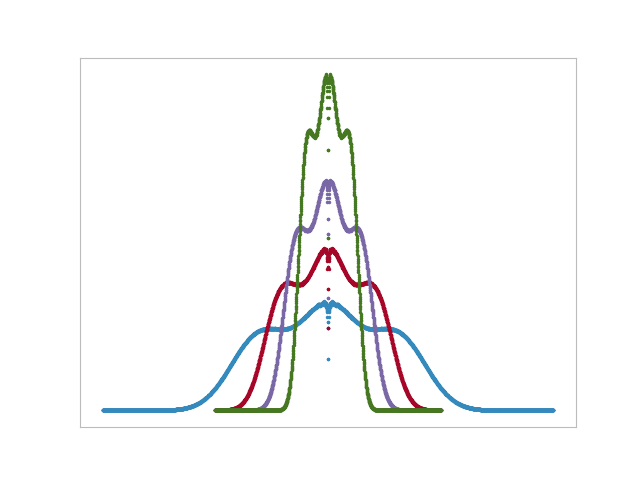
\includegraphics[scale=0.6]{Images/art_white.png}
	\caption{One-body density plots for a two-dimensional single quantum dot containing 12 electrons, popularly called an artificial Magnesium atom. The four graphs correspond to four different oscillator frequencies, where the weakest oscillator gives the broadest density distribution. It's quite artistic, isn't it?}
\end{figure}

We are finally ready to discuss the most interesting part of this thesis, namely the results. Since this work, after all, is about physics the physical insight should be our focus, and in this chapter we finally get the opportunity to discuss pure physics. However, we will also use this section for the comparison of restricted Boltzmann machine (RBM) and the standard variational Monte Carlo method (VMC) to see which one that works best and in which situations they differ. Actually, we will look at three versions of the RBM; a Slater determinant consisting of Boltzmann machines only (RBM), a RBM with the simple Jastrow factor described in section \ref{sec:simplejastrow} (RBM+SJ) and a RBM with the Padé-Jastrow factor described in section \ref{sec:padejastrow} (RBM+PJ). The VMC consists of a Slater determinant containing standard single-particle functions and the Padé-Jastrow factor. 

As we can look at various systems, system sizes, system strengths and innumerous hyper-parameter settings by different methods, the number of results we possibly can obtain is uncountable. In total, we have looked at more than 150 different quantum dot systems using four methods, which means that we have generated a large set of results. Just a small subset of those results will be presented and discussed in this chapter, while a larger collection of results is presented in appendix \ref{chp:totalresults}. The results presented above were selected since they describe physical properties and compare the various methods in a good way. Typically, we will choose settings that are comparable to what others have obtained, such that we can benchmark the calculations. Our main focus will be on ground-state energy and electron density calculations. 

Before we move on to the physical results, we will take a quick look at some more technical results, more precisely the computational cost of various wave function structures and the energy convergence using various optimization tools. For validation purposes, we will present a few selected results on the case without repulsive interaction and compare to analytical results. Thereafter, we study the case with repulsive interaction in a much larger scale, where we first look at single quantum dots and then on double quantum dots. We also take a brief look at atoms to demonstrate the flexibility and generality of the code. 

\section{Computational cost}
Many-body quantum simulations are frequently found on lists of the most computationally expensive simulations for scientific purposes, which is caused by the large amount of information that is stored in the wave function. Albeit the VMC method is known to have a high performance-cost ratio, the it is still not cheap. In this section we will find the average cost of VMC and compare the cost to the RBM methods detailed above. In figure \eqref{fig:cpu_time} the CPU-time is plotted as a function of the number of particles for two-dimensional (left) and three-dimensional (right) quantum dots. To obtain accurate times, all the simulations were run on the Abel computer cluster with $M=2^{20}=1,048,576$ Monte Carlo cycles per iteration. The time presented is the average time over at least four independent runs with thousands of iterations each. To see the actual numbers, go to appendix \ref{chp:totalresults}, section \ref{sec:cputime}. 

\begin{figure}[h]
	\centering 
	% This file was created by matplotlib2tikz v0.7.4.
\begin{tikzpicture}[scale=0.9]

\begin{axis}[name=2D, xlabel=$N$, ylabel={CPU-time [s]}, grid=major, 
legend cell align={left},
legend style={at={(1.68,1.10)}, anchor=south east, draw=white!80.0!black},
legend columns = 6, 
clip=false,
xtick=data] 
\addplot[color=color0,mark=oplus*, dashed] coordinates { 
	(2,6.05)
	(6,11.25)
	(12,20.53) 
	(20,38.99) 
	(30,73.73) 
	(42,130.49) 
	(56,213.47)
	(72,360.22)
	(90,856.84) }; 
\addlegendentry{RBM};

\addplot[color=color1,mark=oplus*, dash dot] coordinates { 
	(2,7.12) 
	(6,14.07) 
	(12,28.42) 
	(20,63.27) 
	(30,122.93) 
	(42,199.60)
	(56,349.22)}; 
\addlegendentry{RBM+SJ};

\addplot[color=color2,mark=oplus*, dotted] coordinates { 
	(2,7.26)
	(6,13.50)
	(12,27.68)
	(20,57.09) 
	(30,119.17) 
	(42,212.53) 
	(56,382.13) }; 
\addlegendentry{RBM+PJ};

\addplot[color=color3,mark=oplus*] coordinates { 
	(2,5.11)
	(6,10.51)
	(12,20.85) 
	(20,41.20) 
	(30,76.26) 
	(42,137.39) 
	(56,230.63)
	(72,355.81)
	(90,544.03) }; 
\addlegendentry{VMC};

\node[] at (axis cs: 44,978) {2D};
\end{axis}

\begin{axis}[name=2D, 
xshift=7.9cm, 
xlabel=$N$, 
grid=major, 
clip=false,
xtick=data] 
\addplot[color=color0,mark=oplus*, dashed] coordinates { 
	(2,7.69)
	(8,20.92)
	(20,59.67) 
	(40,171.84) 
	(70,586.39) }; 
%\addlegendentry{RBM};

\addplot[color=color1,mark=oplus*, dash dot] coordinates { 
	(2,8.95)
	(8,26.86)
	(20,94.64) 
	(40,270.92) }; 
%\addlegendentry{RBM+SJ};

\addplot[color=color2,mark=oplus*, dotted] coordinates { 
	(2,8.87)
	(8,26.36)
	(20,91.40) 
	(40,293.25) }; 
%\addlegendentry{RBM+PJ};

\addplot[color=color3,mark=oplus*] coordinates { 
	(2,6.70)
	(8,20.99)
	(20,62.54) 
	(40,185.65) 
	(70,486.02) };
%\addlegendentry{VMC};

\node[] at (axis cs: 35,670) {3D};
\end{axis}
\end{tikzpicture}
	\caption{CPU-time per iteration for $M=2^{20}=1,048,576$ cycles as a function of number of electrons for two- dimensional (left) and three-dimensional (right) quantum dots. The number of processes was 128 and the simulations were performed without a burn-in period. Table with numbers and more information about simulations can be found in appendix \ref{chp:totalresults}, section \ref{sec:cputime}. For abbreviations see the text.}
	\label{fig:cpu_time}
\end{figure} 

Our immediate observation is that the methods are pairwise quite similar, with RBM and VMC as the cheapest methods and RBM+SJ and RBM+PJ are the most expensive ones. This is not surprising, as the RBM requires a neural network, VMC requires a Jastrow factor while RBM+SJ and RBM+SJ requires both a neural network and a Jastrow factor. 

For two-dimensional dots, the RBM is the cheapest among all the methods, but for larger systems ($N=42,56$ with $N$ as the number of electrons), VMC gets cheaper due to an explosion in CPU-time for the RBM. This explosion can be explained by our choice of the number of hidden nodes, $H$, which consequently is set to the number of electrons, i.e., $H=N$ , which was found to give the lowest energies when testing on small quantum dots \cite{nordhagen_computational_2018}. Since the RBM has $N\cdot D\cdot (1+H)+H$ variational parameters with $D$ as the number of dimensions, the number of variational parameters for a dot containing 90 particles in two dimensions is 16,470! On the other hand, VMC has two variational parameters which obviously makes the parameter update simpler. 

We also observe that the RBM+PJ is cheaper than the RBM+SJ for systems up to $N=42$, but after that the RBM+SJ gets slightly cheaper. This might be surprising, as the simple Jastrow contains $N^2$ variational parameters, but a possibility is that BLAS is optimized for large matrix-vector operations and is thus fully utilized first when the matrices get large. The exact same behavior is observed for three-dimensional quantum dots, and the discussion above is describing for them as well.

The standard way of estimating the scaling of a VMC algorithm, is to fit the power function $f(x)=ax^b$. As all the simulations were performed with the same hyper-parameters and with all the outer factors as similar as possible, we fix the first parameter $a$ and focus on the second parameter $b$ only. It is this latter parameter that specifies the scaling, i.e., we say that the method scales as $N^b$. For comparison reasons, we set $a=0.5$ as this was found to be a good average value. In table \eqref{tab:cputimefit}, the optimal $b$ from linear regression is presented for our four methods in two and three dimensions. We want to emphasize that the we only did the regression for CPU-times up to 56 particles in two dimensions and 40 particles in three dimensions, partly because we only have data for all methods in this interval and partly because the CPU-time for the RBM explodes for large dots. We believe that this was the best way to do it in order to make the various methods comparable. 

\begin{table}
	\caption{The scaling for two- and three-dimensional quantum dot system as a function of the dot size. The numbers presented in the table are the optimal $b$-value found from linear regression on the function $f(N)=0.5N^b$. For the script, see \lstinline|cost_power_reg.py|. For abbreviations see the text.}
	\begin{tabularx}{\textwidth}{CCCCC} \hline\hline
		\label{tab:cputimefit}
		\makecell{\\ \phantom{=}} & RBM & RBM+SJ & RBM+PJ & VMC \\ \hline \\
		2D & 1.498 & 1.639 & 1.621 & 1.515 \\ 
		3D & 1.584 & 1.710 & 1.729 & 1.605 \\ \hline\hline
	\end{tabularx}
\end{table}

The numbers in the table matches our impression from figure \eqref{fig:cpu_time}, where RBM and VMC pairwise were found to be more expensive than RBM+SJ and RBM+PJ. For all the methods, the scaling was found to be between linear and quadratic as a function of number of particles, which is surprising as the update of the Slater matrix scales as $\sim N^2$. 

\newpage
\section{Energy convergence}
We want our calculations to converge fast and to be stable, and that is what the optimization tool is responsible for. In figure \eqref{fig:convergenceoptimization}, we compare standard gradient descent (GD) to stochastic gradient descent (SGD) and ADAM for quantum dots with two interacting electrons in two and three dimensions. The gradient descent methods are plain, i.e., without momentum and adaptive learning rate, while the ADAM optimizer has momentum and adaptivity by nature. The frequency $\omega=1.0$ is used for the two-dimensional case since we know that the exact energy is $E=3.0$ for this case \cite{taut_two_1993}. Similarly, we use the frequency $\omega=0.5$ for the three-dimensional case since the exact energy is $E=2.0$ \cite{taut_two_1994}. 

\begin{figure}[h]
	\centering 
	\subfloat{{\begin{tikzpicture} [scale=0.9, spy using outlines=
	{rectangle, magnification=8,size=2cm, height=1cm, connect spies}]
	\begin{axis} [name=2D, 
	xlabel=Iteration, 
	ylabel={Energy [Ha]}, 
	grid=major, 
	clip=false,
	every axis plot/.append style={thick},
	legend cell align={left},
	legend style={at={(1.45,1.1)}, anchor=south east, draw=white!80.0!black},
	legend columns = 6
	]
	
	\addplot[color2] table [x expr=\coordindex+1, 
	y index=0, 
	mark=none] {/home/evenmn/VMC/data/int1/quantumdot/energy/VMC/2D/2P/1.000000w/GD_MC16777216.dat};
	\addlegendentry{GD};
	
	\addplot[color1] table [x expr=\coordindex+1, 
	y index=0, 
	mark=none] {/home/evenmn/VMC/data/int1/quantumdot/energy/VMC/2D/2P/1.000000w/SGD_MC16777216.dat}; 
	\addlegendentry{SGD};
	
	\addplot[color0] table [x expr=\coordindex+1, 
	y index=0, 
	mark=none, 
	color=blue] {/home/evenmn/VMC/data/int1/quantumdot/energy/VMC/2D/2P/1.000000w/ADAM_MC16777216.dat}; 
	\addlegendentry{ADAM};
	
	\addplot [dashed,mark=none,black] coordinates {(0,3) (100,3)};
	\addlegendentry{Exact};
	
	\node[] at (axis cs: 50,3.178) {2D, $\omega=1.0$};
	\coordinate (spypoint1) at (axis cs:75,2.995001);
	\coordinate (magnifyglass1) at (axis cs:50,3.1);
	\end{axis}
	\spy [size=2.0cm] on (spypoint1)
	in node[fill=white] at (magnifyglass1);
	
	\begin{axis} [name=3D, 
	xshift=7.9cm, 
	xlabel=Iteration, 
	grid=major, 
	clip=false,
	every axis plot/.append style={thick}]	
	\addplot[color2] table[x expr=\coordindex+1, y index=0, mark=none] {/home/evenmn/VMC/data/int1/quantumdot/energy/VMC/3D/2P/0.500000w/GD_MC16777216.dat};  
	%\addlegendentry{GD};
	
	\addplot[color1] table[x expr=\coordindex+1, y index=0, mark=none] {/home/evenmn/VMC/data/int1/quantumdot/energy/VMC/3D/2P/0.500000w/SGD_MC16777216.dat};  
	%\addlegendentry{SGD};
	
	\addplot[color0] table[x expr=\coordindex+1, y index=0, mark=none] {/home/evenmn/VMC/data/int1/quantumdot/energy/VMC/3D/2P/0.500000w/ADAM_MC16777216.dat}; 
	%\addlegendentry{ADAM};
	
	\addplot+ [dashed,mark=none,color=black] coordinates {(0,2) (100,2)};
	%\addlegendentry{Exact};
	
	\node[] at (axis cs: 50,2.1355) {3D, $\omega=0.5$};
	\coordinate (spypoint2) at (axis cs:75,1.997);
	\coordinate (magnifyglass2) at (axis cs:50,2.077);
	\end{axis} 
	\spy [size=2.0cm] on (spypoint2)
	in node[fill=white] at (magnifyglass2);
\end{tikzpicture}}}
	\caption{Energy convergence for circular quantum dots where we use the optimization tools gradient descent (GD), stochastic gradient descent with 10 batches (SGD) and the ADAM optimizer. The left-hand side plot shows a two-dimensional quantum dot of frequency $\omega=1.0$ containing two interacting electrons with exact energy $E=3.0$. The right-hand side plot shows a three-dimensional quantum dot of frequency $\omega=0.5$ containing two interacting electrons with exact energy $E=2.0$. To obtain the graphs, we use VMC detailed in the introductory words of this chapter, the learning rate was set to $\eta=0.5$ and the number of Metropolis steps used for each iteration was $M=2^{24}=16,777,216$. All energies are given in units of $\hbar$ (Hartree units).}
	\label{fig:convergenceoptimization}
\end{figure} 

The first thing we observe, is that all the three optimization tools manage to converge to the exact energy (see spy window). The stochastic and non-stochastic gradient descent methods behave similarly, but we observe that the SGD converges faster than the GD. The ADAM optimizer, on the other hand, fluctuates much more. This behavior can be described by the momentum, as discussed in section \ref{sec:momentum}. It is also important to remember that this is the case when we use standard variational Monte-Carlo wave function, which is equipped with two variational parameters only. The ADAM optimizer is known to be good at machine learning problems where we have many variational parameters, so we will stick to it even though gradient descent seems like a clever choice seen from the figure. Another point is that the circular quantum dots have neat potentials without local minima. When we move on to more complex systems, ADAM generally works better according to the literature. 

\newpage
\section{No repulsive interaction} \label{sec:norepulsive}
We start with the non-interacting case in order to validate the implemented code. For this case, we know the exact energy and the exact electron density for both single quantum dots, double quantum dots and atoms, which makes it a good test for all the systems. The physical significance is though limited as such systems do not appear in the real world. We will start with the single quantum dot, and then move on to atoms. 

\subsection{Quantum dots}
Quantum dots is the system we will keep most of the attention on, and for that reason we will also validate the implemented quantum dot code thoroughly. As we use the harmonic oscillator potential to describe the attraction in the circular quantum dots, the system has well-known analytical results for the most common observable. The quantum dot has analytical ground state energies given by equation \eqref{eq:HOenergies} and a number of particles given by the magic numbers in equation \eqref{eq:HOclosedshell}. For some selected number of electrons and for frequencies $\omega=0.5$ and $\omega=1.0$, we compare our obtained energies to the analytical energies in table \eqref{tab:quantumdotswointeraction}. We observe that both the standard VMC, with $\alpha=1$, and standard RBM, with all parameters set to zero, are able to reproduce the analytical expression. This is as expected, since the exact wave functions are found when the parameters have these particular values.

\begin{table}[h]
	\caption{Energy of circular quantum dots of frequency $\omega=0.5$ and $\omega=1.0$ containing $N$ non-interacting particles. Exact values are obtained by $E=\omega(n+1/2)$, and all values are given in units of $\hbar$. The standard error is zero down to machine precision, and for abbreviations see the text.}
	\label{tab:quantumdotswointeraction}
	\begin{tabularx}{\textwidth}{r|rR{2cm}R{2cm}R{2cm}:R{2cm}R{2cm}R{2cm}} \hline\hline
		&& \multicolumn{3}{c}{$\omega=0.5$}&\multicolumn{3}{c}{$\omega=1.0$}\\ \hline
		\makecell{\\ \phantom{=}}& $N$ & \multicolumn{1}{c}{RBM} & \multicolumn{1}{c}{VMC} & \multicolumn{1}{c}{Exact} & \multicolumn{1}{c}{RBM} & \multicolumn{1}{c}{VMC} & \multicolumn{1}{c}{Exact} \\ \hline \\
		
		\parbox[t]{2mm}{\multirow{3}{*}{\rotatebox[origin=c]{90}{2D}}}
		&2 & 1.0 & 1.0 & 1 & 2.0 & 2.0 & 2\\
		%&6 & 5.0 & 5.0 & 5 & 10.0 & 10.0 & 10 \\
		&12 & 14.0 & 14.0 & 14 & 28.0 & 28.0 & 28\\
		%&20 & 30.0 & 30.0 & 30 & 60.0 & 60.0 & 60\\
		&30 & 55.0 & 55.0 & 55 & 110.0 & 110.0 & 110\\ \hline \\
		
		\parbox[t]{2mm}{\multirow{3}{*}{\rotatebox[origin=c]{90}{3D}}}
		&2 & 1.5 & 1.5 & 1.5 & 3.0 & 3.0 & 3 \\
		%&8 & 9.0 & 9.0 & 9 & 18.0 & 18.0 & 18 \\
		&20 & 30.0 & 30.0 & 30 & 60.0 & 60.0 & 60 \\
		%&40 & 75.0 & 75.0 & 75 & 150.0 & 150.0 & 150 \\
		&70 & 157.5 & 157.5 & 157.5 & 315.0 & 315.0 & 315 \\ \hline\hline
	\end{tabularx}
\end{table}

We will also focus on the electron density throughout the results, and comparing the obtained densities to the analytical ones is a good indicator on whether the implementation is correct or not. In figure \eqref{fig:OB_nointeraction} the one-body densities are plotted for quantum dots of two non-interacting electrons in two and three dimensions with frequency $\omega=1.0$. In part (left) the spatial one-body density distribution simulated using VMC is given, while in (middle) and (right) the radial density profile for VMC, RBM and the exact profile is given in two and three dimensions respectively. We observe that both VMC and RBM are more or less able to reproduce the exact distribution, which indicates that we have done the implementation correctly. However, the densities get noisy when they approach $r=0$, most notably in three dimensions, which is caused by the way we calculate the radial one-body densities. In section \ref{sec:electrondensityimplementation}, we saw that the innermost bins are also the smallest, which means that particles are less likely to be observed there when the number of Monte Carlo cycles is finite. This effect is not found in part (a), because that one-body density was computed by dividing the space into equally sized squares. Apart from this noise, the density plot in two and three dimensions are identical, which can be explained mathematically by the fact that the non-interacting electron densities are separable. The analytical one-body densities are found from the definition of one-body density in equation \eqref{eq:electron_density}.

\begin{figure}
	\centering
	\captionsetup[subfigure]{labelformat=empty}
	\subfloat[2D]{\includegraphics[width=7cm]{/home/evenmn/VMC/plots/int0/onebody/2D/2P/GD_MC2pow30_w1p0.png}}
	\subfloat[3D]{\includegraphics[width=7cm]{/home/evenmn/VMC/plots/int0/onebody/3D/2P/GD_MC2pow30_w1p0.png}}\\
	
	\subfloat[VMC]{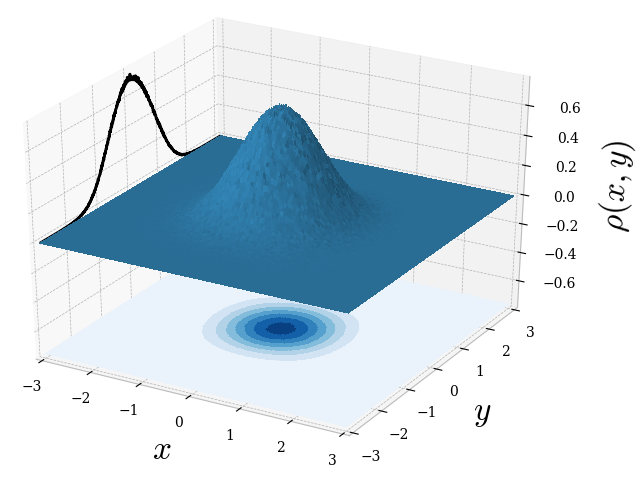
\includegraphics[width=7cm]{/home/evenmn/VMC/plots/int0/onebody2/2D/2P/1.000000w/VMC_GD_MC2pow30_blue_small.png}}
	\subfloat[RBM]{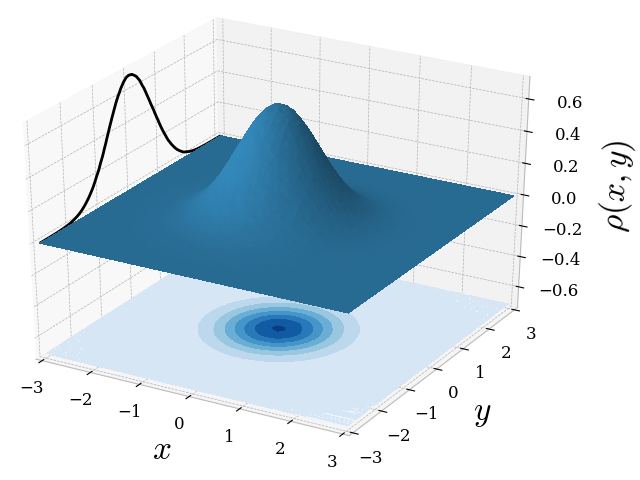
\includegraphics[width=7cm]{/home/evenmn/VMC/plots/int0/onebody2/2D/2P/1.000000w/RBM_ADAM_MC268435456.png}}
	\caption{The one-body density for a quantum dot of frequency $\omega=1.0$ with two non-interacting electrons. The upper plots give the radial density profiles of two-dimensional (left) and three-dimensional (right) dots produced using VMC and RBM and compared to the analytical case, while the lower present the spatial one-body distribution for the two-dimensional case produced with VMC (left) and RBM (right). The exact solution was found from the definition of one-body density found in equation \eqref{eq:electron_density}. For abbreviations see the text.}
	\label{fig:OB_nointeraction}
\end{figure}

Also the two-body density is interesting to examine as it might provides information about the interactions that the one-body density cannot give us. The radial two-body density profile is computed in the same way as the radial one-body density profile, and we expect therefore to observe the same effect where the density drops in the center. In figure \eqref{fig:TB_nointeraction}, we plot the obtained two-body density using VMC (left) and the exact density found from equation \eqref{eq:electron_density} (right). We observe that the simulated two-body density is similar to the exact one, but apparently not as smooth. We also get a cross on the simulated density profile, which occurs since we in practice only simulate one quadrant and add the three other quadrants to make the plot more intuitive and illustrative. As we have seen before, the electron densities are separable without interaction, which means that the radial two-body density presented here simply is the radial one-body density rotated in space. 

As discussed before, the electron densities should be normalized such that the integral over the density function $\rho$ is the number of particles. For the one-body density, this corresponds to $\int dr\rho(r)=N$ for the radial density profile and $\int dxdy\rho(x,y)=N$ for the spatial density distribution and for the two-body radial density profile the normalization condition is $\int dr_idr_j\rho(r_i,r_j)=N$. However, there is no standard way of normalizing these densities when they are calculated using bins like us, as the normalization constant depends on the number of bins and so on. This is not very important either, we are only interested in the relative densities and the shapes of the density plots. We have been consequent when normalizing the density plots, such that the various density magnitudes can be compared to each other.

\begin{figure}
	\centering
	\captionsetup[subfigure]{labelformat=empty}
	\subfloat[VMC]{{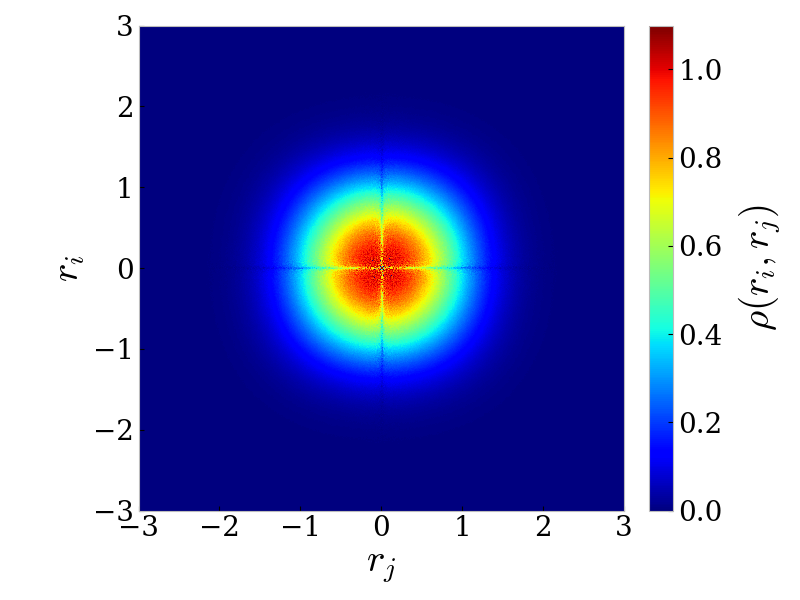
\includegraphics[width=7cm]{/home/evenmn/VMC/plots/int0/twobody/VMC/2D/2P/1.000000w/VMC_GD_MC2pow30.png} }}
	\subfloat[Exact]{{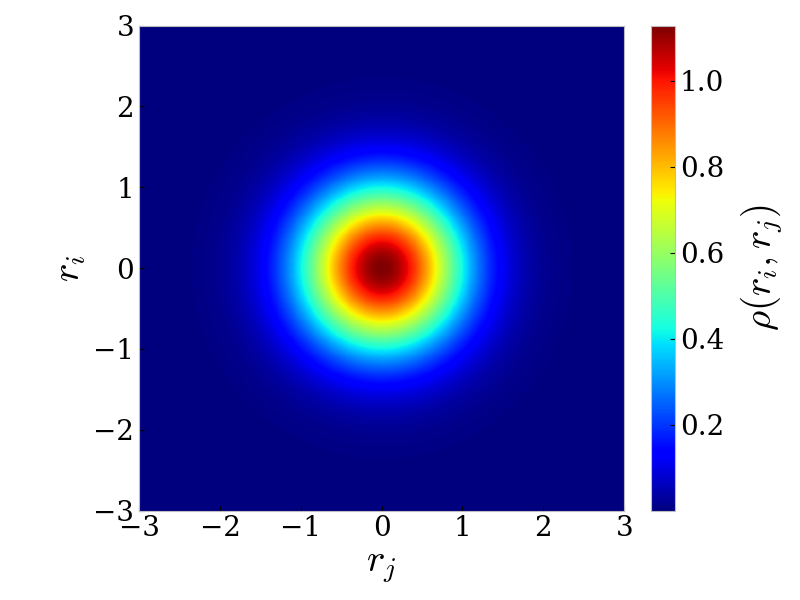
\includegraphics[width=7cm]{/home/evenmn/VMC/plots/int0/twobody/VMC/2D/2P/1.000000w/exact.png}}}
	\caption{Two-body density for a two-dimensional quantum dot with frequency $\omega=1.0$ containing two non-interacting electrons. We use VMC for the simulation (a) and compare it to the exact solution was found from the definition of two-body density found in equation \eqref{eq:electron_density}. For abbreviations see the text.}%
	\label{fig:TB_nointeraction}
\end{figure}

\iffalse
\newpage
\subsection{Double quantum dots}
For the double quantum dots, we can also find analytical energies without interaction, as explained in section \ref{sec:doubledots}. We first find the matrix 
\begin{equation*}
\hat{h}_{\nu\lambda}=\mel{\phi_{\nu}^{\text{HO}}(x)}{\hat{\mathcal{H}}_{\text{HO}}}{\phi_{\lambda}^{\text{HO}}(x)}+\mel{\phi_{\nu}^{\text{HO}}(x)}{\hat{\mathcal{H}}_{\text{+}}}{\phi_{\lambda}^{\text{HO}}(x)}
\end{equation*}
for a satisfying number of harmonic oscillator functions (basis functions). All the symbols are detailed in section \ref{sec:doubledots}. The energies are the eigenvalues of the matrix, which were obtained by the script \texttt{doublewell\_functions.py}. For one particle in one-dimensional potentials, we get the energy $E=0.3095$ for $\omega=1.0$ and $b=2$, and $E=0.1916$ for $\omega=0.5$ and $b=4$. This gives the analytical energies presented in table \eqref{tab:doubledotswointeraction}. 
\begin{table} [H]
	\caption{Energy of double quantum dots of frequency $\omega$ and with a splitting parameter $b$ containing two non-interacting electrons. The methods used were detailed in the introductory words of this chapter.}
	\label{tab:doubledotswointeraction}
	\begin{tabularx}{\textwidth}{lrrrR{3.5cm}R{3.5cm}R{3.5cm}} \hline\hline
		D & $\omega$ & $b$ & \makecell{\\ \phantom{=}} & RBM & VMC & Exact \\ \hline \\
		
		2D & 0.5 & 4.0 && - & - & 0.8832 \\
		& 1.0 & 2.0 && - & 1.6207(2) & 1.619 \\
		3D & 0.5 & 4.0 && - & - & 1.3832 \\
		& 1.0 & 2.0 && - & - & 2.619 \\ \hline\hline
	\end{tabularx}
\end{table}

The VMC reproduces the energies perfectly, while the RBM does not...
\fi

\subsection{Atoms}
Lastly, we will look at atoms with non-interacting electrons in order to validate our code. The analytical energy of those atoms is given by the Bohr formula presented in equation \eqref{eq:bohrformula}. In table \eqref{tab:atomswointeraction}, the lowest closed-shell atoms He, Be and Ne are listed with their exact energy and the obtained energy from the code. In addition, we added calculations of the Hydrogen ground-state energy as another simple test. We see that all energies are reproduced to machine precision, with the variational parameter $\alpha=1.0$. This gives the exact wave function, and is a good indication. 

\begin{table}[H]
	\caption{Energy of neutral atoms with atomic number $Z$ and non-interacting atoms surrounding it. The energy is given in units of $\hbar$, and the variance is zero to machine precision for all listed results. For abbreviations see the text.}
	\label{tab:atomswointeraction}
	\begin{tabularx}{\textwidth}{R{3.5cm}lrrR{2.5cm}R{2.5cm}} \hline\hline
		& Atom & $Z$ & \makecell{\\ \phantom{=}} & VMC & Exact \\ \hline \\
		
		& H & 1 && -0.5 & -0.5 \\
		& He & 2 && -4.0 & -4 \\
		& Be & 4 && -20.0 & -20 \\
		& Ne & 10 && -200.0 & -200 \\ \hline\hline
	\end{tabularx}
\end{table}

\cleardoublepage
\section{Quantum dots}
We now move on to the more interesting case with repulsive interaction, where we no longer have analytical results, apart from a few semi-analytical energies and wave functions  for the two- and three-dimensional single quantum dots. We will for this system calculate the ground state energy, the one-body density and the two-body density. 

The simulations are dependent on an array of parameters and factors, and in order to achieve good results these parameters need to be reasonable. Firstly, the simulations are very sensitive about the learning rate, which need to be small to avoid the quantum force to explode, but still large enough for the system to converge in an acceptable number of iterations. Appropriate learning rates were found to be between $\eta=0.5$ and 0.00001 dependent on the system, where large systems and/or systems with low frequency needed the smallest learning rates. To get good statistics, we always try to keep the acceptance ratio around 0.99. This is controlled by the step length, which again is very dependent on the frequency of the oscillator where high frequency dots are more narrow, and therefore need a lower step length. Also the initial particle configurations and initial parameters are crucial to make the simulations converge rapidly. Lastly, the statistical error naturally also depends on the number of Monte Carlo cycles, where a high number of cycles is preferred. We have applied an adaptive step number, which means that the number cycles per iteration is increased for the last iterations. Firstly, this makes the final energy more accurate due to better statistics. Secondly, we get less noisy electron density plots by using this technique. All results below are produced using $2^{20}=1,048,576$ number of steps per iteration until the energy has converged. Then we run 10 more iterations with the number of steps increased to $2^{24}=16,777,216$ and for the very last iteration we run $2^{28}=268,435,456$ steps. This technique also provides smooth electron density plots.

Initially, we look at two-dimensional quantum dots with up to $N=56$ electrons and three-dimensional quantum dots with up to $N=40$ electrons and frequencies spanning from  $\omega=0.1$ to $\omega=1.0$. For those systems, we will compute the ground state energy, the one-body density and the two-body density. After that, we move on to some special cases where the dots have low frequency ($\omega=0.01$) and large dots ($N>$56) to test how far we can go. For those systems, we will typically focus on either the ground-state energy or the one-body density dependent on what we want to investigate. For instance, we will focus on the one-body density for low frequency dots because of the search for Wigner crystals. We also have a thorough discussion of how the energy is distributed between kinetic and potential energy, and compare this to the virial theorem.

\subsection{Ground-state energy} \label{sec:groundstateenergy}
The ground-state energy is a natural start as it is what we try to minimize, and it can easily be compared to benchmarks. By exploiting the symmetry of quantum dots with two electrons, M.Taut was able to obtain semi-analytical energies for some specific frequencies $\omega$. More specifically, he found the energy to be $E=3$ for the frequency $\omega=1$ and $E=2/3$ for the frequency $\omega=1/6$ for the two-dimensional case, and $E=2$ for the frequency $\omega=1/2$ and $E=1/2$ for the frequency $\omega=1/10$ for the three-dimensional case \cite{taut_two_1993,taut_two_1994}.

For other references, we need to rely on what researchers have found before us. Since diffusion Monte-Carlo (DMC) is known to give very accurate results, we will mainly compare our results to J. Høgberget's DMC computations, which exist for quantum dots containing maximum 56 electrons in two dimensions and maximum 20 particles in three dimensions \cite{hogberget_quantum_2013}. Comparing the energy to the Hartree-Fock limit is also interesting, mainly because the Boltzmann machines need to be better to have any significance as Hartree-Fock is much cheaper. We use A.Mariadason's computations for this for quantum dots up to 20 electrons in two dimensions, and up to 8 particles in three dimensions \cite{mariadason_quantum_2018}.

\afterpage{
	\begin{landscape}
		\begin{table}
			\captionsetup{width=0.9\hsize}
			\caption{The ground state energy of two-dimensional circular quantum dots of frequency $\omega$ containing $N$ electrons. The Hartree-Fock limit results (HF) are taken from Ref.\cite{mariadason_quantum_2018}, the diffusion Monte Carlo (DMC) results are taken from Ref.\cite{hogberget_quantum_2013} and semi-analytical results (Exact) are taken from Ref.\cite{taut_two_1994}. For other abbreviations see the text. The energy is given in units of $\hbar$, and the numbers in parenthesis are the statistical uncertainties in the last digit.}
			\begin{tabularx}{\hsize}{llR{2.65cm}R{2.65cm}R{2.65cm}R{2.65cm}R{2.65cm}R{2.65cm}R{2.65cm}} \hline\hline
				\label{tab:quantumdotswinteraction2D1}
				\makecell{\\ $N$ \\ \phantom{=}} & $\omega$ & \multicolumn{1}{c}{RBM} & \multicolumn{1}{c}{RBM+SJ} & \multicolumn{1}{c}{RBM+PJ} & \multicolumn{1}{c}{\makecell{HF \\ (Ref.\cite{mariadason_quantum_2018})}} & \multicolumn{1}{c}{VMC} & \multicolumn{1}{c}{\makecell{DMC \\ (Ref.\cite{hogberget_quantum_2013})}} & \multicolumn{1}{c}{\makecell{Exact \\ (Ref.\cite{taut_two_1994})}} \\ \hline \\
				2 & 0.1 & 0.4728(1) & 0.44856(1) & 0.440975(8) & 0.525635 & 0.44129(1) & 0.44079(1) \\ 
				& 1/6 & 0.7036(1) & 0.67684(7) & 0.66715(6) & 0.768675 & 0.66710(1) & - & 2/3 \\
				& 0.28 & 1.07050(4) & 1.03470(7) & 1.021668(7) & 1.14171 & 1.02192(1) & 1.02164(1) \\
				& 0.5 & 1.72293(7) & 1.67739(9) & 1.659637(6) & 1.79974 & 1.65974(1) & 1.65977(1)  \\
				& 1.0 & 3.0803(2) & 3.02108(5) & 2.999587(5) & 3.16190 & 2.99936(1) & 3.00000(1) & 3.0 \\ 
				\hline \\
				
				6 & 0.1 & 3.697(1) & 3.63825(9) & 3.5700(2) & 3.85238 & 3.5695(1) & 3.55385(5) \\ 
				& 0.28 & 7.9273(9) & 7.7313(2) & 7.6203(2) & 8.01957 & 7.6219(1) & 7.60019(6) \\
				& 0.5 & 12.241(1) & 11.9659(5) & 11.8074(2) & 12.2713 & 11.8104(2) & 11.78484(6) \\
				& 1.0 & 20.716(1) & 20.3393(8) & 20.1832(2) & 20.7192 & 20.1918(2) & 20.15932(8) \\ \hline \\
				
				12 & 0.1 & 12.679(1) & 12.5964(7) & 12.3416(4) & 12.9247 & 12.29962(9) & 12.26984(8) \\ 
				& 0.28 & 26.389(2) & 26.051(1) & 25.7331(5) & 26.5500 & 25.7049(4) & 25.63577(9) \\
				& 0.5 & 40.440(3) & 39.6340(7) & 39.2743(6) & 40.2161 & 39.2421(5) & 39.1596(1) \\
				& 1.0 & 67.632(3) & 66.1898(8) & 65.7911(7) & 66.9113 & 65.7026(4) & 65.7001(1) \\ \hline
			\end{tabularx}
		\end{table}
		
		\begin{table}
			\label{tab:quantumdotswinteraction2D2}
			\begin{tabularx}{\hsize}{llR{2.65cm}R{2.65cm}R{2.65cm}R{2.65cm}R{2.65cm}R{2.65cm}R{2.65cm}} \\
				20 & 0.1 & 30.824(2) & 30.567(3) & 30.1553(9) & 31.1902 & 30.0403(2) & 29.9779(1) \\ 
				& 0.28 & 63.788(4) & 62.786(3) & 62.148(1) & 63.5390 & 62.0755(7) & 61.9268(1) \\
				& 0.5 & 96.491(4) & 94.920(4) & 94.104(1) & 95.7328 & 94.0433(9) & 93.8752(1) \\
				& 1.0 & 159.645(5) & 156.816(4) & 156.104(1) & 158.004 & 155.8900(4) & 155.8822(1) & \phantom{=} \\ 
				\hline \\
				
				30 & 0.1 & 61.829(5) & 61.198(2) & 60.774(2) & & 60.585(1) & 60.4205(2) \\ 
				& 0.28 & 126.958(6) & 126.067(5) & 124.437(2) & & 124.195(2) & 123.9683(2) \\
				& 0.5 & 191.495(7) & 188.995(5) & 187.488(2) & & 187.325(3) & 187.0426(2) \\
				& 1.0 & 315.364(8) & 309.997(6) & 308.989(2) & & 308.576(1) & 308.5627(2) \\ \hline \\
				
				42 & 0.1 & 109.892(6) & 109.48(2) & 108.753(6) & &  107.928(2) & 107.6389(2) \\ 
				& 0.28 & 224.462(8) & 224.184(9) & 222.200(5) & & 220.224(2) & 219.8426(2) \\
				& 0.5 & 337.523(8) & 333.582(9) & 331.410(3) & & 331.276(3) & 330.6306(2) \\
				& 1.0 & 553.40(1) & 545.817(9) & 543.746(3) & & 542.977(2) & 542.9428(8) \\ \hline \\
				
				56 & 0.1 & - & 179.59(1) & - & & 176.774(3) & 175.9553(7) \\ 
				& 0.28 & 364.85(1) & 364.165(9) & 359.83(2) & & 359.63(1) & 358.145(2) \\
				& 0.5 & 547.46(1) & 545.74(1) & 538.810(7) & & 538.686(9) & 537.353(2) \\
				& 1.0 & 894.12(2) & 882.93(1) & 881.010(5) & & 879.514(3) & 879.3986(6) \\ \hline\hline
			\end{tabularx}
		\end{table}
		
		\begin{table}
			\captionsetup{width=0.9\hsize}
			\caption{The ground state energy of two-dimensional circular quantum dots of frequency $\omega$ containing $N$ electrons.  The Hartree-Fock limit results (HF) are taken from Ref.\cite{mariadason_quantum_2018}, the diffusion Monte Carlo (DMC) results are taken from Ref.\cite{hogberget_quantum_2013} and semi-analytical results (Exact) are taken from Ref.\cite{taut_two_1993}. For other abbreviations see the text. The energy is given in units of $\hbar$, and the numbers in parenthesis are the statistical uncertainties in the last digit.} 
			\begin{tabularx}{\hsize}{llR{2.65cm}R{2.65cm}R{2.65cm}R{2.65cm}R{2.65cm}R{2.65cm}R{2.65cm}} \hline\hline
				\label{tab:quantumdotswinteraction3D1}
				\makecell{\\ $N$ \\ \phantom{=}} & $\omega$ & \multicolumn{1}{c}{RBM} & \multicolumn{1}{c}{RBM+SJ} & \multicolumn{1}{c}{RBM+PJ} & \multicolumn{1}{c}{\makecell{HF \\ (Ref.\cite{mariadason_quantum_2018})}} & \multicolumn{1}{c}{VMC} & \multicolumn{1}{c}{\makecell{DMC \\ (Ref.\cite{hogberget_quantum_2013})}} & \multicolumn{1}{c}{\makecell{Exact \\ (Ref.\cite{taut_two_1993})}} \\ \hline \\
				2 & 0.1 & 0.5177(1) & 0.50214(3) & 0.500080(6) & 0.529065 & 0.500083(7) & 0.499997(3) & 0.5 \\
				& 0.28 & 1.2261(1) & 1.20475(4) & 1.201710(6) & 1.23722 & 1.201752(6) & 1.201725(2) \\
				& 0.5 & 2.0269(1) & 2.00371(4) & 1.999912(5) & 2.03851 & 1.999977(5) & 2.000000(2) & 2.0 \\
				& 1.0 & 3.7574(1) & 3.73543(4) & 3.729827(5) & 3.77157 & 3.730030(5) & 3.730123(3) \\ 
				\hline \\
				
				8 & 0.1 & 5.8910(6) & 5.7498(4) & 5.718(4) & 5.86255 & 5.7126(1) & 5.7028(1) \\ 
				& 0.28 & 12.650(1) & 12.2492(4) & 12.2056(2) & 12.3987 & 12.2050(2) & 12.1927(1) \\
				& 0.5 & 19.487(2) & 19.0241(4) & 18.9747(2) & 19.1916 & 18.9759(1) & 18.9611(1) \\
				& 1.0 & 33.302(1) & 32.7159(6) & 32.6820(2) & 32.9246 & 32.6863(2) & 32.6680(1) \\ 
				\hline \\
				
				20 & 0.1 & 27.813(2) & 27.470(1) & 27.3382(8) & & 27.3144(5) & 27.2717(2) \\ 
				& 0.28 & 57.700(4) & 56.600(1) & 56.4477(6) & & 56.4297(5) & 56.3868(2) \\
				& 0.5 & 87.840(4) & 85.893(1) & 85.7153(6) & & 85.7161(5) & 85.6555(2) \\
				& 1.0 & 146.292(4) & 143.209(2) & 142.9409(6) & & 142.9560(7) & 142.8875(2) \\ \hline \\
				
				40 & 0.1 & 89.45(8) & 89.618(4) & 88.596(4) & & 88.182(1) \\ 
				& 0.28 & 182.714(6) & 181.877(4) & 179.630(1) & & 179.567(1) \\
				& 0.5 & 275.262(7) & 271.030(4) & 269.782(2) & & 269.746(1) \\
				& 1.0 & 452.732(8) & 442.874(4) & 442.630(1) & & 442.602(2) \\ \hline\hline
			\end{tabularx}
		\end{table}
	\end{landscape}
}

Ground state energy computations of two- and three dimensional quantum dots are found in tables \eqref{tab:quantumdotswinteraction2D1} and \eqref{tab:quantumdotswinteraction3D1} respectively. They are computed by a restricted Boltzmann machine (RBM), restricted Boltzmann machine with a simple Jastrow factor (RBM+SJ), restricted Boltzmann machine with Padé-Jastrow factor (RBM+PJ) and standard variational Monte-Carlo (VMC). In addition, the Hartree-Fock limit (HF) and diffusion Monte-Carlo (DMC) are present for reference purposes. The exact values are found in the last column with the same name. 

We observe that the method where less physical intuition is used, RBM, is the one that gives the highest energies among our implemented methods. This is as expected as no Jastrow factor is added to account for the correlations. For small quantum dots (less than 8 particles), the RBM energy is lower than the Hartree-Fock limit, and for low frequencies ($\omega=0.1$ and $0.28$), the RBM energy is also lower. However, for higher frequencies and larger dots, the Hartree-Fock limit is lower than the obtained energy with the RBMs. It is apparent that the mean field approximation works better than the RBM when the interactions get less important. 

When we add more intuition in form of a simple Jastrow factor the energy drops significantly, especially for high frequencies. It is therefore lower than the HF-limit for all simulations, and surprisingly close to the reference considering the simple form of the Jastrow factor. The statistical errors for RBM+SJ is in general smaller than for RBM, which is a good indication that the method provides a better ground state estimate as the true ground state obey a zero-variance property. 

Furthermore, we added a more complex Jastrow factor in the form of a Padé-Jastrow factor, and we observe that the energy drops further. Actually, the RBM+PJ provides energies completely on par with VMC, in many cases even lower. Notably, RBM+PJ provides the lowest energies among our implemented methods for dots with two electrons, and the statistical errors are also the lowest. This hints that RBM+PJ actually is able to obtain a better ground state estimate than VMC for the smallest dots, which makes sense as the former method is more flexible than VMC. However, for large dots RBM+PJ provides slightly higher energies than VMC, which we suspect is a result of the large number of variational parameters. If we recall that the number of hidden nodes is set to the number of particles, the number of variational parameters increases rapidly as the number of particles increases. Possibly, the model has not fully converged. 

We also see that all the methods are able to obtain energies closer to the reference energy in three dimensions compared to two dimensions. This is a well-known concept, and occurs because we have more degrees of freedom. One can imagine that the electrons can move in the space instead of just in the plane, which makes it easier to form a configuration that minimizes the energy. 

Efforts was made to reproduce the results using a partly restricted Boltzmann machine and a deep belief network, but due to convergence problems and fluctuations, the methods were not investigated further. 

\subsection{One-body density} \label{sec:onebodyresults}
Another quantity of particular interest is the one-body density. For all the systems presented in tables \eqref{tab:quantumdotswinteraction2D1} and \eqref{tab:quantumdotswinteraction3D1} we have also calculated the one-body density. However, since those plots would occupy tens of pages, we will not present all of them here. Instead, we select a few illustrative plots that might be interesting for the reader and give a representative picture of the density. The total collection of one-body density plots can be found in section \ref{sec:onebody} in appendix \ref{chp:totalresults}. 

\begin{figure}
	\centering
	\captionsetup[subfigure]{labelformat=empty}
	\subfloat{\raisebox{2.5cm}{\rotatebox[origin=t]{90}{$N=2$}}}\hspace{0.1cm}
	\subfloat{{\includegraphics[width=7.8cm]{/home/evenmn/VMC/plots/int1/onebody2/2D/2P/1.000000w/RBM_ADAM_MC2pow28_smooth_blue.png}}}\hspace{-0.0cm}
	\subfloat{{\includegraphics[width=7.8cm]{/home/evenmn/VMC/plots/int1/onebody2/2D/2P/1.000000w/VMC_ADAM_MC1048576.png}}}\\
	
	\subfloat{\raisebox{2.5cm}{\rotatebox[origin=t]{90}{$N=6$}}}\hspace{0.05cm}
	\subfloat{{\includegraphics[width=7.8cm]{/home/evenmn/VMC/plots/int1/onebody2/2D/6P/1.000000w/RBM_ADAM_MC2pow28_smooth_blue.png}}}\hspace{-0.0cm}
	\subfloat{{\includegraphics[width=7.8cm]{/home/evenmn/VMC/plots/int1/onebody2/2D/6P/1.000000w/VMC_ADAM_MC2pow28_smooth_blue.png}}}\\
	
	\subfloat{\raisebox{2.5cm}{\rotatebox[origin=t]{90}{$N=12$}}}\hspace{0.1cm}
	\subfloat[RBM]{{\includegraphics[width=7.8cm]{/home/evenmn/VMC/plots/int1/onebody2/2D/12P/1.000000w/RBM_ADAM_MC2pow28_smooth_blue.png}}}\hspace{-0.0cm}
	\subfloat[VMC]{{\includegraphics[width=7.8cm]{/home/evenmn/VMC/plots/int1/onebody2/2D/12P/1.000000w/VMC_ADAM_MC2pow28_smooth_blue.png}}}
	
	\caption{One-body density plots for two-dimensional circular quantum dots with frequency $\omega=1.0$. The plots present quantum dots containing 2, 6 and 12 electrons, and were all obtained using RBM and VMC. ADAM optimizer was used, and after convergence the number of Monte-Carlo cycles was $M=2^{28}=268,435,456$. The plots are noise-reduced using a Savitzky-Golay filter, and for abbreviations see the text.}
	\label{fig:OB_interaction_1p0w1}
\end{figure}
\begin{figure}
	\centering
	\captionsetup[subfigure]{labelformat=empty}
	\subfloat{\raisebox{2.5cm}{\rotatebox[origin=t]{90}{$N=20$}}}\hspace{0.1cm}
	\subfloat{{\includegraphics[width=7.8cm]{/home/evenmn/VMC/plots/int1/onebody2/2D/20P/1.000000w/RBM_ADAM_MC2pow28_smooth_blue.png}}}\hspace{-0.0cm}
	\subfloat{{\includegraphics[width=7.8cm]{/home/evenmn/VMC/plots/int1/onebody2/2D/20P/1.000000w/VMC_ADAM_MC2pow28_smooth_blue.png}}}\\
	
	\subfloat{\raisebox{2.5cm}{\rotatebox[origin=t]{90}{$N=30$}}}\hspace{0.1cm}
	\subfloat{{\includegraphics[width=7.8cm]{/home/evenmn/VMC/plots/int1/onebody2/2D/30P/1.000000w/RBM_ADAM_MC2pow28_smooth_blue.png}}}\hspace{-0.0cm}
	\subfloat{{\includegraphics[width=7.8cm]{/home/evenmn/VMC/plots/int1/onebody2/2D/30P/1.000000w/VMC_ADAM_MC2pow28_smooth_blue.png}}}\\
	
	\subfloat{\raisebox{2.5cm}{\rotatebox[origin=t]{90}{$N=42$}}}\hspace{0.1cm}
	\subfloat[RBM]{{\includegraphics[width=7.8cm]{/home/evenmn/VMC/plots/int1/onebody2/2D/42P/1.000000w/RBM_ADAM_MC2pow28_smooth_blue.png}}}\hspace{-0.0cm}
	\subfloat[VMC]{{\includegraphics[width=7.8cm]{/home/evenmn/VMC/plots/int1/onebody2/2D/42P/1.000000w/VMC_ADAM_MC2pow28_smooth_blue.png}}}
	
	\caption{One-body density plots for two-dimensional circular quantum dots with frequency $\omega=1.0$. The plots present quantum dots containing 20, 30 and 42 electrons, and were all obtained using RBM and VMC, detailed in the introductory words of this chapter. ADAM optimizer was used, and after convergence the number of Monte-Carlo cycles was $M=2^{28}=268,435,456$. The plots are noise-reduced using a Savitzky-Golay filter, and for abbreviations see the text.}
	\label{fig:OB_interaction_1p0w2}
\end{figure}

We have computed the one-body density in two different ways: by dividing the space into annuluses and obtaining the radial density profile, as discussed in section \ref{sec:electrondensityimplementation}, and by dividing the space into a grid of equally sized bins and obtaining the density profile throughout the space. The former is computational beneficial as the density typically is stored in $n$ bins compared to $n^2$ bins for the second method, but the latter is obviously able to store more information. The second method is thereby able to give more informative plots, but when we want to compare the various wave function choices a radial density profile is more convenient. In other words, there are pros and cons associated with both methods, and we will therefore present both to give an as comprehensive description of the results as possible. 

We will start with spatial density profiles for two-dimensional quantum dots of frequency $\omega=1.0$. In figure \eqref{fig:OB_interaction_1p0w1} and \eqref{fig:OB_interaction_1p0w2}, dots of sizes $N=2$, 6, 12, 20, 30 and 42 are presented, produced with RBM and VMC. To maximize the amount of information in the plot, we have included a contour plot and a cross section line plot in addition to a 3D plot of the density. What we observe is that the density gets a wave shape, with more peaks as the number of particles increases. For odd number of shells (2, 12 and 30 electrons) the density has its maximum in the center of the dot, while for even number of shells (6, 20 and 42 electrons) the highest density is found at a ridge that encircles the center. This result follows directly from the Pauli principle, as the electrons are forced to distribute over multiple shells. Even when we remove the interaction between the electrons, we get the same characteristic wave shape, though narrower. The RBM provides sharper and more distinct peaks than the VMC, but at least the extrema seem to be located at the same radii. These differences are caused by the ways the methods model the correlations, where the VMC uses the Padé-Jastrow factor and the RBM needs to find the best way to account for the correlations itself. To connect the observations to something everyone is familiar with, the density plots behave like a water ripple if one sees it from the smallest to the largest dots. J.Høgberget points this out in his master thesis, and his one-body densities are consistent with what we have obtained \cite{hogberget_quantum_2013}. One-body density plots for the same systems using RBM+SJ and RBM+PJ were generated, but in order to limit us to a few plots we decided to keep the extremes here, and placed the others in appendix \ref{chp:totalresults}.

In figure \eqref{fig:OB_interaction_23D}, we stick to frequency $\omega=1.0$ for small two- and three-dimensional quantum dots and compare the results obtained by VMC, RBM, RBM+SJ and RBM+PJ. We investigate dots of 2, 6 and 12 electrons in two dimensions and 2, 8 and 20 particles in three dimensions, which corresponds to one shell ($S=1$), two shells ($S=2$) and three shells ($S=3$) respectively. For all the cases, we immediately see that the density plots are identical in two and three dimensions for the same closed shell. The same phenomenon was observed for quantum dots with non-interacting electrons in figure \eqref{fig:OB_nointeraction}, but in that case it can be easily be explained as the wave function is trivially separable. This is not the situation when we look at the interacting case, and it was therefore not obvious to us that the same phenomenon would occur in that case. However, what is most interesting for us is to analyze the performance of the Boltzmann machines. We observe that all the methods give quite similar radial density profiles, but RBM is always the guy standing out. Apparently, the RBM tends to over-exaggerate the ripples discussed above and gives an even more wavy density plot, as also observed in figures \eqref{fig:OB_interaction_1p0w1} and \eqref{fig:OB_interaction_1p0w2}. Further, the RBM+SJ is more similar to the VMC and RBM+PJ, which are almost identical. This is consistent with the energy analysis in section \ref{sec:groundstateenergy}, where we found VMC and RBM+PJ to be most accurate, followed by RBM+SJ and RBM. We also observe some noise close to $r=0$, which is caused by the fact that the number of Monte Carlo cycles is finite and we in practice have bins of different sizes.

\afterpage{
\begin{figure}[H]
	\centering
	\captionsetup[subfigure]{labelformat=empty}
	\subfloat{\raisebox{1.5cm}{\rotatebox[origin=t]{90}{$S=1$}}}\hspace{0.1cm}
	\subfloat{{\includegraphics[width=5.1cm]{/home/evenmn/VMC/plots/int1/onebody2/2D/2P/1.000000w/VMC_ADAM_MC2pow28_smooth_blue_small.png}}}\hspace{-0.0cm}
	\subfloat{{\includegraphics[width=5.1cm]{/home/evenmn/VMC/plots/int1/onebody/2D/2P/1.000000w/ADAM_MC1048576.png}}}\hspace{-0.5cm}
	\subfloat{{\includegraphics[width=5.1cm]{/home/evenmn/VMC/plots/int1/onebody/3D/2P/1.000000w/ADAM_MC1048576.png}}}\\ [-0.2cm]
	
	\subfloat{\raisebox{1.5cm}{\rotatebox[origin=t]{90}{$S=2$}}}\hspace{0.1cm}
	\subfloat{{\includegraphics[width=5.1cm]{/home/evenmn/VMC/plots/int1/onebody2/2D/6P/1.000000w/VMC_ADAM_MC2pow28_smooth_blue_small.png}}}\hspace{-0.0cm}
	\subfloat{{\includegraphics[width=5.1cm]{/home/evenmn/VMC/plots/int1/onebody/2D/6P/1.000000w/ADAM_MC1048576.png}}}\hspace{-0.5cm}
	\subfloat{{\includegraphics[width=5.1cm]{/home/evenmn/VMC/plots/int1/onebody/3D/8P/1.000000w/ADAM_MC1048576.png}}}\\ [-0.2cm]
	
	\subfloat{\raisebox{1.5cm}{\rotatebox[origin=t]{90}{$S=3$}}}\hspace{0.1cm}
	\subfloat[VMC, 2D]{{\includegraphics[width=5.1cm]{/home/evenmn/VMC/plots/int1/onebody2/2D/12P/1.000000w/VMC_ADAM_MC2pow28_smooth_blue_small.png}}}\hspace{-0.0cm}
	\subfloat[2D]{{\includegraphics[width=5.1cm]{/home/evenmn/VMC/plots/int1/onebody/2D/12P/1.000000w/ADAM_MC1048576.png}}}\hspace{-0.5cm}
	\subfloat[3D]{{\includegraphics[width=5.1cm]{/home/evenmn/VMC/plots/int1/onebody/3D/20P/1.000000w/ADAM_MC1048576.png}}}
	
	\caption{One-body density plot for small circular quantum dots with frequency $\omega=1.0$. We look at the three lowest shells $S=1$, 2 and 3 corresponding to 2, 6 and 12 particles in two dimensions and 2, 8 and 20 particles in three dimensions. In the first column, the density profile for the space are presented for the two-dimensional dots using VMC where the graph on the $yz$-plane represent the cross section through $x=0$. In the second column the corresponding radial density profiles are obtained using the same methods as in figure \eqref{fig:cpu_time}. On the right-hand side, the radial density profiles for the three-dimensional dots are given using the same methods. ADAM optimizer was used, and after convergence the number of Monte-Carlo cycles was $M=2^{28}=268,435,456$. The surface plots are noise-reduced using a Savitzky-Golay filter, and for abbreviations see the text.}
	\label{fig:OB_interaction_23D}
\end{figure}
}

We now move on to larger dots, containing $N=20$ and $N=42$ electrons with frequencies $\omega=0.1$ and $\omega=0.5$ in addition to the above-studied frequency $\omega=1.0$ to see if we can observe something interesting. In figure \eqref{fig:OB_interaction} we plot the radial density profile to again compare all the methods. What we see, is that the ripples discussed above are conserved for lower frequencies, and they possibly become more significant as the frequency drops. Also the density distribution gets broader as the frequency drops, since the force pushing the electrons towards the center of the dot gets weaker. Moreover, all the methods VMC, RBM+PJ and RBM+SJ appear to give quite similar density plots, but for lower frequencies the difference gets more and more visible. In particular, the peaks for frequency $\omega=0.1$ do no longer match for the various methods. Especially RBM and RBM+SJ differ from VMC and RBM+PJ, which is again a clear indication that the final result really depends on way the methods account for the correlations. RBM+SJ tends to slightly over-exaggerate the oscillations in the density plots, and RBM takes the over-exaggerations to the next level. This trend was also observed in the plots in figures (\ref{fig:OB_interaction_1p0w1}, \ref{fig:OB_interaction_1p0w2}, \ref{fig:OB_interaction_23D}), and physically, this means that the method is capable of finding the most likely places to find the electrons, but fails to determine the actual density there. We have also seen that the one-body density is shape-invariant for the frequencies $\omega=0.28$, 0.5 and 1.0 except for their radial extent. For that reason, 

\begin{figure}
	\centering
	\captionsetup[subfigure]{labelformat=empty}
	\subfloat{\raisebox{3cm}{\rotatebox[origin=t]{90}{$\omega=0.1$}}}\hspace{0.1cm}
	\subfloat{{\includegraphics[width=8cm]{/home/evenmn/VMC/plots/int1/onebody/2D/20P/0.100000w/ADAM_MC1048576.png}}}\hspace{-0.5cm}
	\subfloat{{\includegraphics[width=8cm]{/home/evenmn/VMC/plots/int1/onebody/2D/42P/0.100000w/ADAM_MC1048576.png}}}\\
	
	\subfloat{\raisebox{3cm}{\rotatebox[origin=t]{90}{$\omega=0.5$}}}\hspace{0.1cm}
	\subfloat{{\includegraphics[width=8cm]{/home/evenmn/VMC/plots/int1/onebody/2D/20P/0.500000w/ADAM_MC1048576.png}}}\hspace{-0.5cm}
	\subfloat{{\includegraphics[width=8cm]{/home/evenmn/VMC/plots/int1/onebody/2D/42P/0.500000w/ADAM_MC1048576.png}}}\\
	
	\subfloat{\raisebox{3cm}{\rotatebox[origin=t]{90}{$\omega=1.0$}}}\hspace{0.1cm}
	\subfloat[20P]{{\includegraphics[width=8cm]{/home/evenmn/VMC/plots/int1/onebody/2D/20P/1.000000w/ADAM_MC1048576.png}}}\hspace{-0.5cm}
	\subfloat[42P]{{\includegraphics[width=8cm]{/home/evenmn/VMC/plots/int1/onebody/2D/42P/1.000000w/ADAM_MC1048576.png}}}
	
	\caption{One-body density plot for two-dimensional circular quantum dots of the oscillator frequencies $\omega=0.1$, 0.5 and 1.0 with $N=20$ and 42 interacting electrons. ADAM optimizer was used, and after convergence the number of Monte-Carlo cycles was $M=2^{28}=268,435,456$. For abbreviations see the text.}
	\label{fig:OB_interaction}
\end{figure}

\newpage
\subsection{Two-body density}
We have on multiple occasions in this thesis discussed the electron density, and we have also mentioned the two-body density. The two-body density is interesting because it gives the probability of finding two particles at certain relative distances from the center of the dot. Unlike the one-body density, this density therefore gives the information of how the particles distribute pairwise, and it is therefore very informative when we want to study the interactions between electrons. Similarly to the one-body density, we can both plot the radial two-body density profile and the actual two-body density distribution throughout the space. However, since the latter results in a higher-dimensional object, we stick to the radial density profile. Also for this quantity it would be convenient to have references to benchmark our results to, but for some reason it is hard to find papers that discuss the two-body density for quantum dots. Nevertheless, someone needs to be the first and we will use the plots to discuss the physics and compare the various methods in the best possible way. Again, we will emphasize that a negative radial distance does not make sense, so all the quadrants are the same and presented in this way to make it more illustrative and intuitive.We will focus on the two-dimensional case, as the three-dimensional case becomes similar in the same way as for the one-body density. 

In figure \eqref{fig:TB_interaction_2P} we plot the two-body density for a two-dimensional quantum dot with two electrons at various frequencies. For frequency $\omega=1.0$, the density plots for all the methods give quite similar results, but the RBM provides a higher two-body density in the middle of the quantum dot, compared to the other methods. This can be seen from the magnitude of the density at the center, but also the density itself is narrower than for its fellow methods, making it more compact. This can be explained by the absent of a Jastrow factor. Also the RBM+SJ gives a slightly more narrow distribution than the RBM+PJ and VMC, so it is apparent that the Padé-Jastrow factor results in a more repulsive factor than the simple Jastrow factor. This can also be seen at the density at origin, which is low for RBM+PJ and VMC, but high for RBM and VMC. We know that the potential, and thus the interactions get more dominating as the frequency drops. For VMC and RBM+PJ, we can observe this by a significant circle of higher density at a certain distance from the origin both for $\omega=0.5$ and $\omega=0.1$, which physically means that both particles are less likely to be found in the center of the dot at the same time. If one particle is close to the center, the other particle is probably far from the center, if one particle is in the center the other is far from the center and vice versa. For the RBM+SJ, this behavior can only be observed for $\omega=0.1$, while the RBM is not able to reproduce this phenomenon at all. This indicates that the RBM is not able to model the correlations correctly, and and it needs a Jastrow factor to account for them. The resolutions of the plots gets lower when we decrease the frequency, as the particles spread over a larger area and therefore more bins.

The calculations are repeated for two-dimensional quantum dots of frequency $\omega=0.5$ and an even number of closed shells (6, 20 and 42 particles), which are presented in figure \eqref{fig:TB_interaction_20P}. The first thing we observe, is that the RBM kind of manages to obtain the correct peaks, but they are all circular unlike the density plots from the VMC, and they are also more distinct and higher than for VMC. This is the same effect we saw in the one-body density plots, which we argued was caused by the different approaches to model the correlations. If we now keep our attention on the VMC plots, it is apparent that two particles will not be observed in the middle of the dot at the same time as the density there is almost zero. For 6 particles, a particle pair is most likely to be found at the same radius around $r=2$, which matches the one-body density plot. When we move on to 20 particles, the most probably place is not ambiguous anymore, but an electron pair is likely to be found at the same radius at around $r=1$, which matches the highest peak in the one-body density plot. However, the density is also high along both axis, which means that if one of the electrons move to the center of the dot, the other will also be moves towards the center. This is probably a consequence of the the interactions. For 42 electrons, finding two 

\begin{landscape}
	\begin{figure}
		\centering
		\captionsetup{width=0.9\hsize}
		\captionsetup[subfigure]{labelformat=empty}
		\subfloat{\raisebox{2cm}{\rotatebox[origin=t]{90}{$\omega=0.1$}}}\hspace{0.1cm}
		\subfloat{{\includegraphics[width=5.7cm]{/home/evenmn/VMC/plots/int1/twobody/2D/2P/0.100000w/RBM_ADAM_MC1048576.png}}}
		\subfloat{{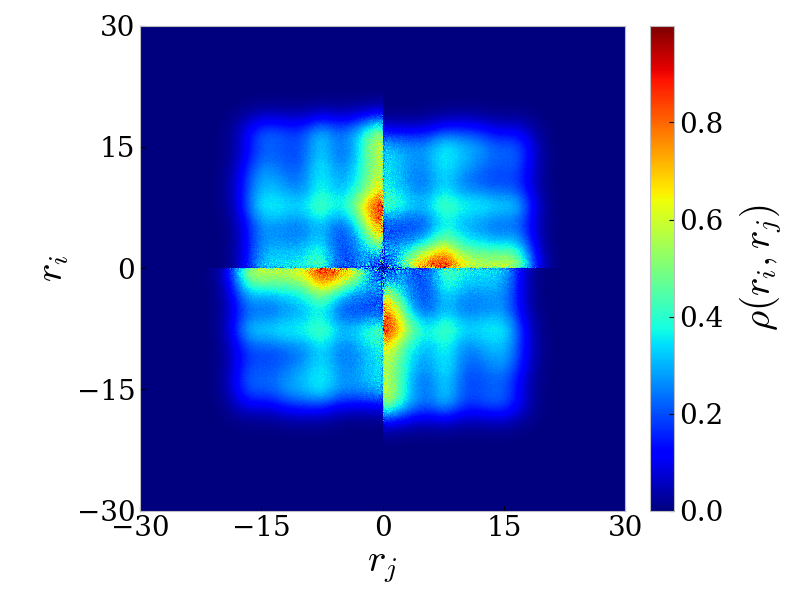
\includegraphics[width=5.7cm]{/home/evenmn/VMC/plots/int1/twobody/2D/2P/0.100000w/RBMSJ_ADAM_MC1048576.png}}}
		\subfloat{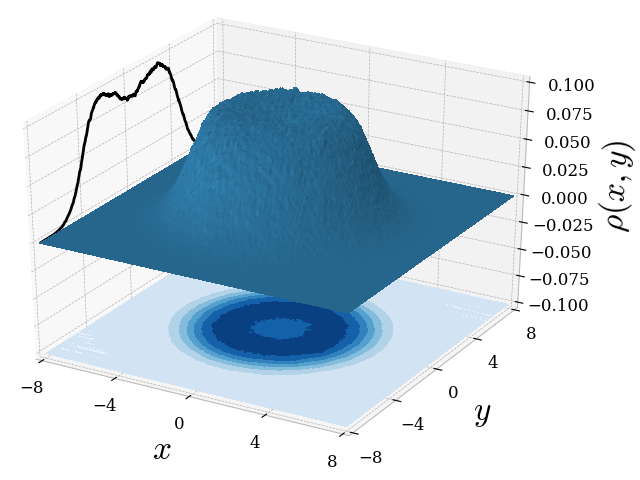
\includegraphics[width=5.7cm]{/home/evenmn/VMC/plots/int1/twobody/2D/2P/0.100000w/RBMPJ_ADAM_MC1048576.png}}
		\subfloat{{\includegraphics[width=5.7cm]{/home/evenmn/VMC/plots/int1/twobody/2D/2P/0.100000w/VMC_ADAM_MC1048576.png}}}
		
		\subfloat{\raisebox{2cm}{\rotatebox[origin=t]{90}{$\omega=0.5$}}}\hspace{0.1cm}
		\subfloat{{\includegraphics[width=5.7cm]{/home/evenmn/VMC/plots/int1/twobody/2D/2P/0.500000w/RBM_ADAM_MC1048576_zoomed.png}}}
		\subfloat{{\includegraphics[width=5.7cm]{/home/evenmn/VMC/plots/int1/twobody/2D/2P/0.500000w/RBMSJ_ADAM_MC1048576_zoomed.png}}}
		\subfloat{\includegraphics[width=5.7cm]{/home/evenmn/VMC/plots/int1/twobody/2D/2P/0.500000w/RBMPJ_ADAM_MC1048576_zoomed.png}}
		\subfloat{{\includegraphics[width=5.7cm]{/home/evenmn/VMC/plots/int1/twobody/2D/2P/0.500000w/VMC_ADAM_MC1048576_zoomed.png}}}\\
		
		\subfloat{\raisebox{2cm}{\rotatebox[origin=t]{90}{$\omega=1.0$}}}\hspace{0.1cm}
		\subfloat[RBM]{{\includegraphics[width=5.7cm]{/home/evenmn/VMC/plots/int1/twobody/2D/2P/1.000000w/RBM_ADAM_MC1048576_zoomed.png}}}
		\subfloat[RBM+SJ]{{\includegraphics[width=5.7cm]{/home/evenmn/VMC/plots/int1/twobody/2D/2P/1.000000w/RBMSJ_ADAM_MC1048576_zoomed.png}}}
		\subfloat[RBM+PJ]{{\includegraphics[width=5.7cm]{/home/evenmn/VMC/plots/int1/twobody/2D/2P/1.000000w/RBMPJ_ADAM_MC1048576_zoomed.png}}}
		\subfloat[VMC]{{\includegraphics[width=5.7cm]{/home/evenmn/VMC/plots/int1/twobody/2D/2P/1.000000w/VMC_ADAM_MC1048576_zoomed.png}}}\\
		
		\caption{Two-body density plots for two-dimensional circular quantum dots of oscillator frequencies $\omega=0.1$, 0.5 and 1.0 with $N=2$ electrons. The ADAM optimizer was used, and after convergence the number of Monte-Carlo cycles was $M=2^{28}=268,435,456$. For abbreviations see the text.}%
		\label{fig:TB_interaction_2P}
	\end{figure}
\end{landscape}
\begin{figure}[H]
	\centering
	\captionsetup{width=0.9\hsize}
	\captionsetup[subfigure]{labelformat=empty}
	\subfloat{\raisebox{2.5cm}{\rotatebox[origin=t]{90}{$N=6$}}}\hspace{0.1cm}
	\subfloat{{\includegraphics[width=7cm]{/home/evenmn/VMC/plots/int1/twobody/2D/6P/0.500000w/RBM_ADAM_MC1048576.png}}}
	\subfloat{{\includegraphics[width=7cm]{/home/evenmn/VMC/plots/int1/twobody/2D/6P/0.500000w/VMC_ADAM_MC1048576.png}}}\\
	
	\subfloat{\raisebox{2.5cm}{\rotatebox[origin=t]{90}{$N=20$}}}\hspace{0.1cm}
	\subfloat{{\includegraphics[width=7cm]{/home/evenmn/VMC/plots/int1/twobody/2D/20P/0.500000w/RBM_ADAM_MC1048576.png}}}
	\subfloat{{\includegraphics[width=7cm]{/home/evenmn/VMC/plots/int1/twobody/2D/20P/0.500000w/VMC_ADAM_MC1048576.png}}}\\
	
	\subfloat{\raisebox{2.5cm}{\rotatebox[origin=t]{90}{$N=42$}}}\hspace{0.1cm}
	\subfloat[RBM]{\includegraphics[width=7cm]{/home/evenmn/VMC/plots/int1/twobody/2D/42P/0.500000w/RBM_ADAM_MC1048576.png}}
	\subfloat[VMC]{{\includegraphics[width=7cm]{/home/evenmn/VMC/plots/int1/twobody/2D/42P/0.500000w/VMC_ADAM_MC1048576.png}}}
	
	\caption{Two-body density plots for two-dimensional circular quantum dots with an even number of closed shells ($N=6$, 20 and 42 electrons) and oscillator frequency $\omega=0.5$. The ADAM optimizer was used, and after convergence the number of Monte-Carlo cycles was $M=2^{28}=268,435,456$. For abbreviations see the text.}%
	\label{fig:TB_interaction_20P}
\end{figure}
\noindent
electrons at the same radius is not the most likely case anymore. This is because the electrons now spread over a large area. The density plot clearly has some distinct drops, matching the fluctuations found in the one-body density plots. For dots with an odd number of closed shells, the same tendency was found, but the peaks were found in the intersection between the quadrants, again matching the one-body density. 

\iffalse
\begin{figure}[H]
	\centering 
	\captionsetup[subfigure]{labelformat=empty}
	\subfloat[RBM]{{% This file was created by tikzplotlib v0.8.1.
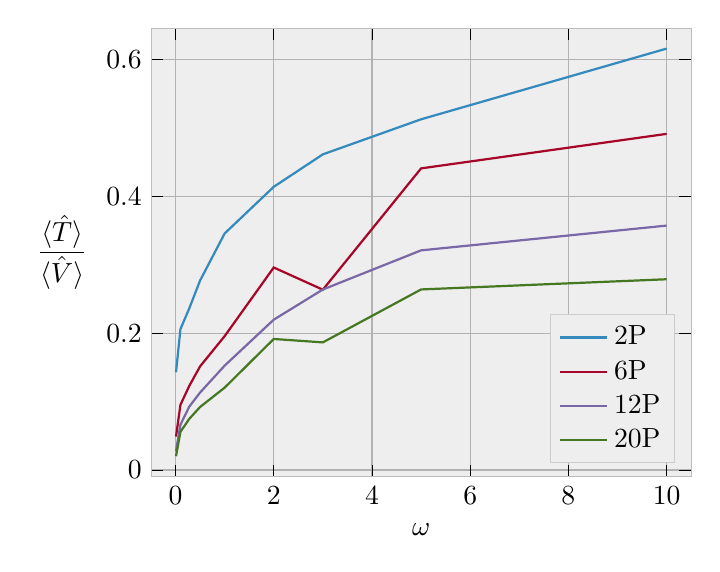
\begin{tikzpicture}

\definecolor{color0}{rgb}{0.203921568627451,0.541176470588235,0.741176470588235}
\definecolor{color1}{rgb}{0.650980392156863,0.0235294117647059,0.156862745098039}
\definecolor{color2}{rgb}{0.47843137254902,0.407843137254902,0.650980392156863}
\definecolor{color3}{rgb}{0.274509803921569,0.470588235294118,0.129411764705882}

\begin{axis}[
axis background/.style={fill=white!93.33333333333333!black},
axis line style={white!73.72549019607844!black},
legend cell align={left},
legend style={at={(0.97,0.03)}, anchor=south east, draw=white!80.0!black, fill=white!93.33333333333333!black},
tick pos=both,
x grid style={white!69.80392156862744!black},
xlabel={\(\displaystyle \omega\)},
xmajorgrids,
xmin=-0.4895, xmax=10.4995,
xtick style={color=black},
y grid style={white!69.80392156862744!black},
ylabel style={rotate=-90.0},
ylabel={\(\displaystyle \frac{\langle\hat{T}\rangle}{\langle\hat{V}\rangle}\)},
ymajorgrids,
ymin=-0.00950153433365221, ymax=0.645814840406007,
ytick style={color=black}
]
\addplot [thick, color0]
table {%
0.01 0.14292980671414
0.1 0.206000508517671
0.28 0.236346842166032
0.5 0.277065579844387
1 0.345784185233727
2 0.41399969664796
3 0.461449773987519
5 0.512681528738802
10 0.616027732463295
};
\addlegendentry{2P}
\addplot [thick, color1]
table {%
0.01 0.0489614243323442
0.1 0.0953652097389264
0.28 0.123020257826888
0.5 0.151552210724365
1 0.195728715728716
2 0.296060131091479
3 0.263623577547628
5 0.440925380415408
10 0.491388484677367
};
\addlegendentry{6P}
\addplot [thick, color2]
table {%
0.01 0.0279279279279279
0.1 0.0663141106354403
0.28 0.0927190456602221
0.5 0.113307273027584
1 0.152620094780267
2 0.21978952717725
3 0.263891885843983
5 0.321107495449782
10 0.357318784099766
};
\addlegendentry{12P}
\addplot [thick, color3]
table {%
0.01 0.0202855736090596
0.1 0.0558188176084186
0.28 0.0748673013733255
0.5 0.092181964299863
1 0.120447174205168
2 0.191577362501107
3 0.186589637000426
5 0.263982205508037
10 0.278872126802915
};
\addlegendentry{20P}
\end{axis}

\end{tikzpicture}}}
	\subfloat[RBM+SJ]{{% This file was created by tikzplotlib v0.8.1.
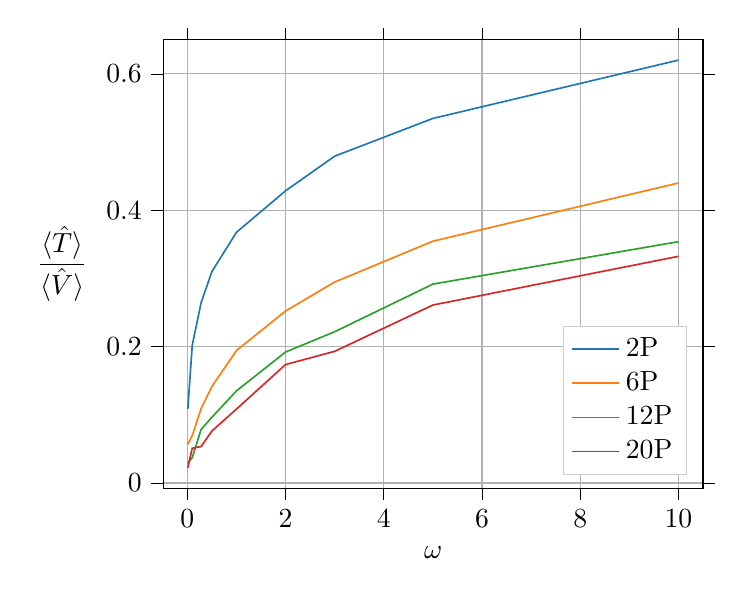
\begin{tikzpicture}

\definecolor{color0}{rgb}{0.12156862745098,0.466666666666667,0.705882352941177}
\definecolor{color1}{rgb}{1,0.498039215686275,0.0549019607843137}
\definecolor{color2}{rgb}{0.172549019607843,0.627450980392157,0.172549019607843}
\definecolor{color3}{rgb}{0.83921568627451,0.152941176470588,0.156862745098039}

\begin{axis}[
legend cell align={left},
legend style={at={(0.97,0.03)}, anchor=south east, draw=white!80.0!black},
tick align=outside,
tick pos=both,
x grid style={white!69.01960784313725!black},
xlabel={\(\displaystyle \omega\)},
xmajorgrids,
xmin=-0.4895, xmax=10.4995,
xtick style={color=black},
y grid style={white!69.01960784313725!black},
ylabel style={rotate=-90.0},
ylabel={\(\displaystyle \frac{\langle\hat{T}\rangle}{\langle\hat{V}\rangle}\)},
ymajorgrids,
ymin=-0.00739548914049018, ymax=0.649881709767761,
ytick style={color=black}
]
\addplot [semithick, color0]
table {%
0.01 0.108705258506407
0.1 0.202009646302251
0.28 0.264296187683284
0.5 0.310018755861207
1 0.367553865652725
2 0.428427393293865
3 0.479188481675393
5 0.534512711346008
10 0.620005473453749
};
\addlegendentry{2P}
\addplot [semithick, color1]
table {%
0.01 0.0567119155354449
0.1 0.0697142186491403
0.28 0.109019214224262
0.5 0.141514485132422
1 0.194234043802478
2 0.252176075603084
3 0.294666494223597
5 0.354539716887567
10 0.439893538370546
};
\addlegendentry{6P}
\addplot [semithick, color2]
table {%
0.01 0.0288659793814433
0.1 0.0372200263504611
0.28 0.0784915858002702
0.5 0.096412072256494
1 0.135095692138839
2 0.192092791484218
3 0.221784714644907
5 0.291641379310345
10 0.353855680855225
};
\addlegendentry{12P}
\addplot [semithick, color3]
table {%
0.01 0.0224807471735212
0.1 0.0510365183964855
0.28 0.0535270823545204
0.5 0.0761996706229769
1 0.108428284656055
2 0.17366909653192
3 0.19307880632568
5 0.260942252768941
10 0.332349732889548
};
\addlegendentry{20P}
\end{axis}

\end{tikzpicture}}}\\
	\subfloat[RBM+PJ]{{% This file was created by tikzplotlib v0.8.1.
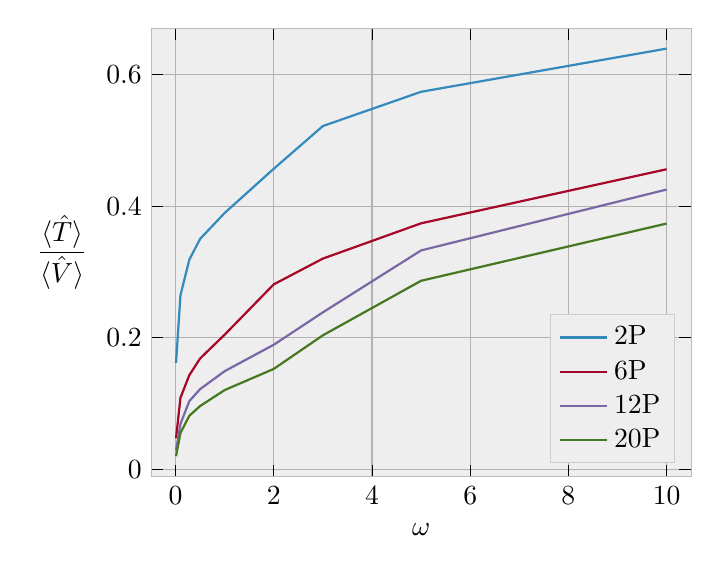
\begin{tikzpicture}

\definecolor{color0}{rgb}{0.203921568627451,0.541176470588235,0.741176470588235}
\definecolor{color1}{rgb}{0.650980392156863,0.0235294117647059,0.156862745098039}
\definecolor{color2}{rgb}{0.47843137254902,0.407843137254902,0.650980392156863}
\definecolor{color3}{rgb}{0.274509803921569,0.470588235294118,0.129411764705882}

\begin{axis}[
axis background/.style={fill=white!93.33333333333333!black},
axis line style={white!73.72549019607844!black},
legend cell align={left},
legend style={at={(0.97,0.03)}, anchor=south east, draw=white!80.0!black, fill=white!93.33333333333333!black},
tick pos=both,
x grid style={white!69.80392156862744!black},
xlabel={\(\displaystyle \omega\)},
xmajorgrids,
xmin=-0.4895, xmax=10.4995,
xtick style={color=black},
y grid style={white!69.80392156862744!black},
ylabel style={rotate=-90.0},
ylabel={\(\displaystyle \frac{\langle\hat{T}\rangle}{\langle\hat{V}\rangle}\)},
ymajorgrids,
ymin=-0.011155128448522, ymax=0.670716886119897,
ytick style={color=black}
]
\addplot [thick, color0]
table {%
0.01 0.161598746081505
0.1 0.264466364626943
0.28 0.318533815178111
0.5 0.350256285086649
1 0.389730328777244
2 0.456965583072599
3 0.52190696776684
5 0.574018126888218
10 0.639722703639515
};
\addlegendentry{2P}
\addplot [thick, color1]
table {%
0.01 0.0468986384266263
0.1 0.108489101409675
0.28 0.142927927927928
0.5 0.168400011874487
1 0.204595643091614
2 0.281150742944763
3 0.320306803143652
5 0.373984932084395
10 0.456212770963223
};
\addlegendentry{6P}
\addplot [thick, color2]
table {%
0.01 0.0287417763157895
0.1 0.0689267491135519
0.28 0.103510351035104
0.5 0.121754035137837
1 0.149081447331657
2 0.189290836653386
3 0.238556500646571
5 0.332749562171629
10 0.425379527774922
};
\addlegendentry{12P}
\addplot [thick, color3]
table {%
0.01 0.0198390540318607
0.1 0.0550696242390316
0.28 0.0812272164373049
0.5 0.0960548685344326
1 0.120346512979882
2 0.152555093728466
3 0.20363356015151
5 0.286590458917023
10 0.373618884667807
};
\addlegendentry{20P}
\end{axis}

\end{tikzpicture}}}
	\subfloat[VMC]{{% This file was created by tikzplotlib v0.8.1.
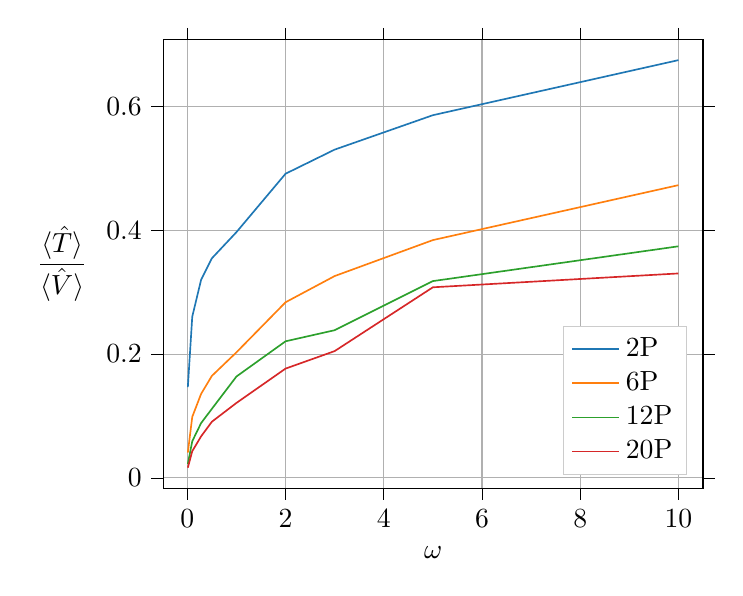
\begin{tikzpicture}

\definecolor{color0}{rgb}{0.12156862745098,0.466666666666667,0.705882352941177}
\definecolor{color1}{rgb}{1,0.498039215686275,0.0549019607843137}
\definecolor{color2}{rgb}{0.172549019607843,0.627450980392157,0.172549019607843}
\definecolor{color3}{rgb}{0.83921568627451,0.152941176470588,0.156862745098039}

\begin{axis}[
legend cell align={left},
legend style={at={(0.97,0.03)}, anchor=south east, draw=white!80.0!black},
tick align=outside,
tick pos=both,
x grid style={white!69.01960784313725!black},
xlabel={\(\displaystyle \omega\)},
xmajorgrids,
xmin=-0.4895, xmax=10.4995,
xtick style={color=black},
y grid style={white!69.01960784313725!black},
ylabel style={rotate=-90.0},
ylabel={\(\displaystyle \frac{\langle\hat{T}\rangle}{\langle\hat{V}\rangle}\)},
ymajorgrids,
ymin=-0.0164668337421715, ymax=0.707728537231861,
ytick style={color=black}
]
\addplot [semithick, color0]
table {%
0.01 0.146594427244582
0.1 0.260418749464423
0.28 0.319901846829394
0.5 0.354717597127
1 0.396972519795063
2 0.491318502441671
3 0.53027950310559
5 0.585870116692034
10 0.67481056582395
};
\addlegendentry{2P}
\addplot [semithick, color1]
table {%
0.01 0.0407722122838402
0.1 0.0985104942450914
0.28 0.135666711367395
0.5 0.164801025691602
1 0.202835527491511
2 0.28369079862382
3 0.326016767506851
5 0.384115256741781
10 0.472868887927304
};
\addlegendentry{6P}
\addplot [semithick, color2]
table {%
0.01 0.0225470925470925
0.1 0.0591952540624194
0.28 0.0885030700825746
0.5 0.111576919808515
1 0.163770657314416
2 0.220633968028807
3 0.238556500646571
5 0.317885405699147
10 0.37406475534662
};
\addlegendentry{12P}
\addplot [semithick, color3]
table {%
0.01 0.0164511376657391
0.1 0.0430938843433643
0.28 0.067074638154502
0.5 0.0907330085826954
1 0.121087634122869
2 0.176534004132603
3 0.20481414099371
5 0.307872099467483
10 0.330233868695407
};
\addlegendentry{20P}
\end{axis}

\end{tikzpicture}}}
	\caption{The kinetic-potential energy ratio $\langle\hat{T}\rangle/\langle\hat{V}\rangle$ plotted as a function of the oscillator frequency for two-dimensional circular quantum dots. The frequencies $\omega=0.01, 0.1, 0.28, 0.5, 1.0, 2.0, 3.0, 5.0, 10.0$ were run. For abbreviations see the text.}
	\label{fig:energysplitVMC2D}
\end{figure}
\fi

\subsection{Energy distribution} \label{sec:energydistributions}
If we now recall the general Hamiltonian presented in chapter \ref{chp:manybody}, the total energy is just the sum of the kinetic, potential and interaction energy. As our methods attempt to solve the Schrödinger equation directly, it is trivial to find the distribution between the various energy sources, which in general is interesting when we want to find the most important contributor to the energy. Additionally, we can use those results to verify the virial theorem presented in section \ref{sec:virial}, and it is also interesting to see if the different methods give different energy distributions. In figure \eqref{fig:energydistribution} we plot the ratio between the kinetic and potential energy as a function of oscillator frequency for two-dimensional quantum dots with up to $N=20$ electrons. The plots are based on the numbers in the tables (\ref{tab:splitfrequencyQDVMC}-\ref{tab:splitfrequencyQDRBMPJ}) in appendix \ref{chp:totalresults}. 

% This file was created by tikzplotlib v0.8.1.
\begin{figure}
\begin{tikzpicture}

\begin{axis}[
legend cell align={left},
legend style={at={(1.7,1.15)}, anchor=south east, draw=white!80.0!black},
legend columns = 4,
title={RBM},
title style={yshift=-1.5ex},
%tick align=outside,
tick pos=both,
x grid style={white!69.01960784313725!black},
%xlabel={\(\displaystyle \omega\)},
width=8cm,
height=5cm,
xmajorgrids,
xmin=-0.4895, xmax=10.4995,
xtick style={color=black},
y grid style={white!69.01960784313725!black},
ylabel style={rotate=-90.0},
ylabel={\(\displaystyle \frac{\langle\hat{T}\rangle}{\langle\hat{V}\rangle}\)},
ymajorgrids,
ymin=-0.03, ymax=0.7,
ytick style={color=black}
]
\addplot [thick, color0]
table {%
	0.01 0.14292980671414
	0.1 0.206000508517671
	0.28 0.236346842166032
	0.5 0.277065579844387
	1 0.345784185233727
	2 0.41399969664796
	3 0.461449773987519
	5 0.512681528738802
	10 0.616027732463295
};
\addlegendentry{$N=2$}
\addplot [thick, color1]
table {%
	0.01 0.0489614243323442
	0.1 0.0953652097389264
	0.28 0.123020257826888
	0.5 0.151552210724365
	1 0.195728715728716
	2 0.296060131091479
	3 0.363623577547628
	5 0.440925380415408
	10 0.491388484677367
};
\addlegendentry{$N=6$}
\addplot [thick, color2]
table {%
	0.01 0.0279279279279279
	0.1 0.0663141106354403
	0.28 0.0927190456602221
	0.5 0.113307273027584
	1 0.152620094780267
	2 0.21978952717725
	3 0.263891885843983
	5 0.321107495449782
	10 0.357318784099766
};
\addlegendentry{$N=12$}
\addplot [thick, color3]
table {%
	0.01 0.0202855736090596
	0.1 0.0558188176084186
	0.28 0.0748673013733255
	0.5 0.092181964299863
	1 0.120447174205168
	2 0.191577362501107
	3 0.2257693437
	5 0.263982205508037
	10 0.278872126802915
};
\addlegendentry{$N=20$}
\end{axis}

\begin{axis}[
xshift=7.7cm,
legend cell align={left},
legend style={at={(0.97,0.03)}, anchor=south east, draw=white!80.0!black},
%tick align=outside,
title={RBM+SJ},
title style={yshift=-1.5ex},
tick pos=both,
x grid style={white!69.01960784313725!black},
%xlabel={\(\displaystyle \omega\)},
xmajorgrids,
width=8cm,
height=5cm,
xmin=-0.4895, xmax=10.4995,
xtick style={color=black},
y grid style={white!69.01960784313725!black},
%ylabel style={rotate=-90.0},
%ylabel={\(\displaystyle \frac{\langle\hat{T}\rangle}{\langle\hat{V}\rangle}\)},
ymajorgrids,
ymin=-0.03, ymax=0.7,
ytick style={color=black}
]
\addplot [thick, color0]
table {%
	0.01 0.108705258506407
	0.1 0.202009646302251
	0.28 0.264296187683284
	0.5 0.310018755861207
	1 0.367553865652725
	2 0.428427393293865
	3 0.479188481675393
	5 0.534512711346008
	10 0.620005473453749
};
%\addlegendentry{2P}
\addplot [thick, color1]
table {%
	0.01 0.0567119155354449
	0.1 0.0697142186491403
	0.28 0.109019214224262
	0.5 0.141514485132422
	1 0.194234043802478
	2 0.252176075603084
	3 0.294666494223597
	5 0.354539716887567
	10 0.439893538370546
};
%\addlegendentry{6P}
\addplot [thick, color2]
table {%
	0.01 0.0288659793814433
	0.1 0.0372200263504611
	0.28 0.0784915858002702
	0.5 0.096412072256494
	1 0.135095692138839
	2 0.192092791484218
	3 0.221784714644907
	5 0.291641379310345
	10 0.353855680855225
};
%\addlegendentry{12P}
\addplot [thick, color3]
table {%
	0.01 0.0224807471735212
	0.1 0.0510365183964855
	0.28 0.0535270823545204
	0.5 0.0761996706229769
	1 0.108428284656055
	2 0.17366909653192
	3 0.19307880632568
	5 0.260942252768941
	10 0.332349732889548
};
%\addlegendentry{20P}
\end{axis}

\end{tikzpicture}

\begin{tikzpicture}

\begin{axis}[
legend cell align={left},
legend style={at={(0.97,1.03)}, anchor=south east, draw=white!80.0!black},
%tick align=outside,
title={RBM+PJ},
title style={yshift=-1.5ex},
tick pos=both,
x grid style={white!69.01960784313725!black},
xlabel={\(\displaystyle \omega\)},
width=8cm,
height=5cm,
xmajorgrids,
xmin=-0.4895, xmax=10.4995,
xtick style={color=black},
y grid style={white!69.01960784313725!black},
ylabel style={rotate=-90.0},
ylabel={\(\displaystyle \frac{\langle\hat{T}\rangle}{\langle\hat{V}\rangle}\)},
ymajorgrids,
ymin=-0.03, ymax=0.75,
ytick style={color=black}
]
\addplot [thick, color0]
table {%
	0.01 0.161598746081505
	0.1 0.264466364626943
	0.28 0.318533815178111
	0.5 0.350256285086649
	1 0.389730328777244
	2 0.456965583072599
	3 0.52190696776684
	5 0.574018126888218
	10 0.639722703639515
};
%\addlegendentry{2P}
\addplot [thick, color1]
table {%
	0.01 0.0468986384266263
	0.1 0.108489101409675
	0.28 0.142927927927928
	0.5 0.168400011874487
	1 0.204595643091614
	2 0.281150742944763
	3 0.320306803143652
	5 0.373984932084395
	10 0.456212770963223
};
%\addlegendentry{6P}
\addplot [thick, color2]
table {%
	0.01 0.0287417763157895
	0.1 0.0689267491135519
	0.28 0.103510351035104
	0.5 0.121754035137837
	1 0.149081447331657
	2 0.189290836653386
	3 0.238556500646571
	5 0.332749562171629
	10 0.425379527774922
};
%\addlegendentry{12P}
\addplot [thick, color3]
table {%
	0.01 0.0198390540318607
	0.1 0.0550696242390316
	0.28 0.0812272164373049
	0.5 0.0960548685344326
	1 0.120346512979882
	2 0.152555093728466
	3 0.20363356015151
	5 0.286590458917023
	10 0.373618884667807
};
%\addlegendentry{20P}
\node[] at (axis cs: 5,-.25) {RBM+PJ};
\end{axis}

\begin{axis}[
xshift=7.7cm,
legend cell align={left},
legend style={at={(0.97,0.03)}, anchor=south east, draw=white!80.0!black},
%tick align=outside,
title={VMC},
title style={yshift=-1.5ex},
tick pos=both,
x grid style={white!69.01960784313725!black},
xlabel={\(\displaystyle \omega\)},
xmajorgrids,
width=8cm,
height=5cm,
xmin=-0.4895, xmax=10.4995,
xtick style={color=black},
y grid style={white!69.01960784313725!black},
%ylabel style={rotate=-90.0},
%ylabel={\(\displaystyle \frac{\langle\hat{T}\rangle}{\langle\hat{V}\rangle}\)},
ymajorgrids,
ymin=-0.03, ymax=0.75,
ytick style={color=black}
]
\addplot [thick, color0]
table {%
	0.01 0.146594427244582
	0.1 0.260418749464423
	0.28 0.319901846829394
	0.5 0.354717597127
	1 0.396972519795063
	2 0.491318502441671
	3 0.53027950310559
	5 0.585870116692034
	10 0.67481056582395
};

\addplot [thick, color1]
table {%
	0.01 0.0407722122838402
	0.1 0.0985104942450914
	0.28 0.135666711367395
	0.5 0.164801025691602
	1 0.202835527491511
	2 0.28369079862382
	3 0.326016767506851
	5 0.384115256741781
	10 0.472868887927304
};

\addplot [thick, color2]
table {%
	0.01 0.0225470925470925
	0.1 0.0591952540624194
	0.28 0.0885030700825746
	0.5 0.111576919808515
	1 0.163770657314416
	2 0.220633968028807
	3 0.238556500646571
	5 0.317885405699147
	10 0.37406475534662
};

\addplot [thick, color3]
table {%
	0.01 0.0164511376657391
	0.1 0.0430938843433643
	0.28 0.067074638154502
	0.5 0.0907330085826954
	1 0.121087634122869
	2 0.176534004132603
	3 0.20481414099371
	5 0.307872099467483
	10 0.330233868695407
};
\end{axis}

\end{tikzpicture}
\caption{The kinetic-potential energy ratio, $\langle\hat{T}\rangle/\langle\hat{V}\rangle$, plotted as a function of the oscillator frequency for two-dimensional quantum dots with $N=2$, 6, 12 and 20 electrons. Simulations with frequencies $\omega=0.01,$ 0.1, 0.28, 0.5, 1.0, 2.0, 3.0, 5.0, 10.0 were performed, see appendix \ref{chp:totalresults} for exact energies. For  abbreviations and description of the natural units used, see the text.}
\label{fig:energydistribution}
\end{figure}

Firstly, the graphs are very similar for the various methods, which means that they all give the same distribution between kinetic and potential energy, although they do not provide the same energy. This is an exciting observation, and means that the obtained kinetic and potential energy are both different for the various methods when the total energy is different. Physically, this indicates that the electron configurations are fundamentally different for the different methods, which is the only factor that can cause a change in potential energy. We see a significant trend where the ratio drops as the frequency drops, implying that the potential energy dominates the kinetic energy at low frequencies, which is a known phenomenon already mentioned several times throughout this thesis. For all the methods the ratio is also lower for larger dots, which is a results of gradually more interaction energy as the number of particles increases.

If we now recall the virial theorem presented in section \ref{sec:virial}, it states that the kinetic energy is related to the potential energies in a certain way. For the interacting quantum dots, the virial theorem reads
\begin{empheq}[box={\mybluebox[5pt]}]{equation}
2\langle \hat{T} \rangle=2\langle \hat{V}_{\text{ext}} \rangle-\langle \hat{V}_{\text{int}} \rangle
\end{empheq}
which can be verified from the 

which in principle can be verified from figure \eqref{fig:energydistribution}. However, 
to do this accurately we will list up the energy distributions for some selected systems.  which for a two-dimensional quantum dot with 20 electrons is given in table \eqref{tab:splitfrequencyQD20P} for some selected frequencies. \textcolor{red}{By doing the math, we see that the virial theorem is satisfied for high frequencies, but as the frequency decreases the theorem gets more and more off. This is the case for all the methods, and is also observed for other system sizes.}

For high frequencies the trap becomes narrow which results in a stronger external force pushing the electrons towards each other. It is therefore natural that both the kinetic energy, external potential energy and interaction energy get larger as the frequency is increased. It is also interesting to see how small the kinetic energy actually is when the frequency is low. We will study this more thoroughly in the next section. For more frequencies and system sizes, please look at appendix \ref{chp:totalresults}.

\iffalse
\begin{figure}  
	\centering 
	\subfloat[$\langle \hat{T} \rangle$]{{% This file was created by tikzplotlib v0.8.1.
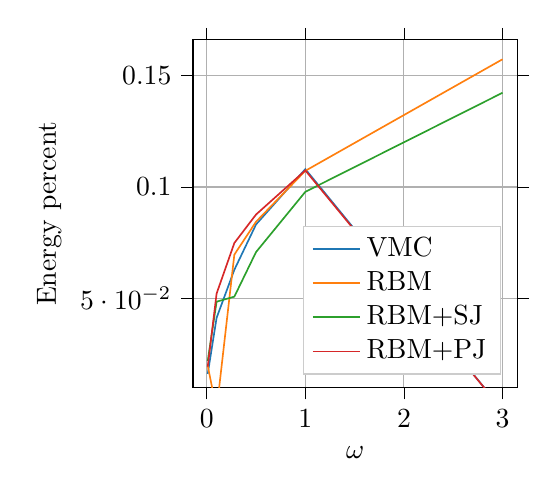
\begin{tikzpicture}

\definecolor{color0}{rgb}{0.12156862745098,0.466666666666667,0.705882352941177}
\definecolor{color1}{rgb}{1,0.498039215686275,0.0549019607843137}
\definecolor{color2}{rgb}{0.172549019607843,0.627450980392157,0.172549019607843}
\definecolor{color3}{rgb}{0.83921568627451,0.152941176470588,0.156862745098039}

\begin{axis}[
legend cell align={left},
legend style={at={(0.34,0.465)}, 
anchor=north west, 
draw=white!80.0!black},
tick align=outside,
tick pos=both,
x grid style={white!69.01960784313725!black},
xlabel={\(\displaystyle \omega\)},
xmajorgrids,
xmin=-0.1395, 
xmax=3.1495,
width=5.7cm,
height=6cm,
xtick style={color=black},
y grid style={white!69.01960784313725!black},
%ylabel={\(\displaystyle \langle\mathcal{T}\rangle/\langle\mathcal{H}\rangle\)},
ylabel={Energy percent},
ymajorgrids,
ymin=0.01, ymax=0.166,
ytick style={color=black}
]
\addplot [semithick, color0]
table {%
0.01 0.0161843567
0.1 0.041314897
0.28 0.062858938
0.5 0.083185086
1 0.108006304
3 0
};
\addlegendentry{VMC}
\addplot [semithick, color1]
table {%
0.01 0.019880972
0.1 0
0.28 0.0696525992
0.5 0.084401654
1 0.107237934
3 0.157246497
};
\addlegendentry{RBM}
\addplot [semithick, color2]
table {%
0.01 0.021990704
0.1 0.048556688
0.28 0.050807505
0.5 0.070803652
1 0.097821651
3 0.142231886
};
\addlegendentry{RBM+SJ}
\addplot [semithick, color3]
table {%
0.01 0.019452496
0.1 0.052195251
0.28 0.074859347
0.5 0.087636916
1 0.10741901
3 0
};
\addlegendentry{RBM+PJ}
\end{axis}

\end{tikzpicture}}}
	\subfloat[$\langle \hat{V}_{\text{ext}} \rangle$]{{% This file was created by tikzplotlib v0.8.1.
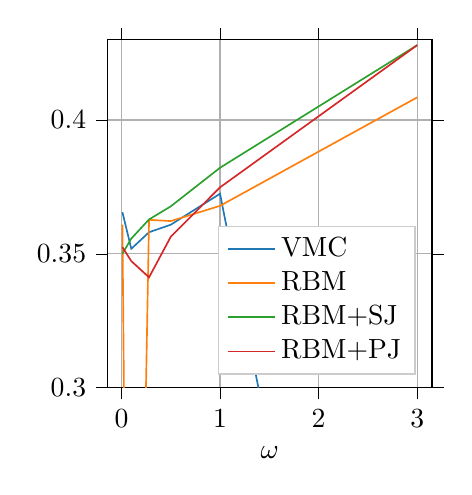
\begin{tikzpicture}

\definecolor{color0}{rgb}{0.12156862745098,0.466666666666667,0.705882352941177}
\definecolor{color1}{rgb}{1,0.498039215686275,0.0549019607843137}
\definecolor{color2}{rgb}{0.172549019607843,0.627450980392157,0.172549019607843}
\definecolor{color3}{rgb}{0.83921568627451,0.152941176470588,0.156862745098039}

\begin{axis}[
legend cell align={left},
legend style={at={(0.34,0.465)}, anchor=north west, draw=white!80.0!black},
tick align=outside,
tick pos=both,
x grid style={white!69.01960784313725!black},
xlabel={\(\displaystyle \omega\)},
xmajorgrids,
xmin=-0.1395, 
xmax=3.1495,
width=5.7cm,
height=6cm,
xtick style={color=black},
y grid style={white!69.01960784313725!black},
%ylabel={\(\displaystyle \langle\mathcal{V}_{ext}\rangle/\langle\mathcal{H}\rangle\)},
ymajorgrids,
ymin=0.30, ymax=0.43,
ytick style={color=black}
]
\addplot [semithick, color0]
table {%
0.01 0.3655571123
0.1 0.351891245
0.28 0.35808008
0.5 0.36087632
1 0.372448783
3 0
};
\addlegendentry{VMC}
\addplot [semithick, color1]
table {%
0.01 0.360945794
0.1 0
0.28 0.3627089294
0.5 0.362241038
1 0.36794137
3 0.408474015
};
\addlegendentry{RBM}
\addplot [semithick, color2]
table {%
0.01 0.350056099
0.1 0.355701411
0.28 0.362851591
0.5 0.36773785
1 0.382174013
3 0.427978032
};
\addlegendentry{RBM+SJ}
\addplot [semithick, color3]
table {%
0.01 0.352495974
0.1 0.347294071
0.28 0.341215239
0.5 0.356358962
1 0.374845451
3 0.4279780324
};
\addlegendentry{RBM+PJ}
\end{axis}

\end{tikzpicture}}}
	\subfloat[$\langle \hat{V}_{\text{int}} \rangle$]{{% This file was created by tikzplotlib v0.8.1.
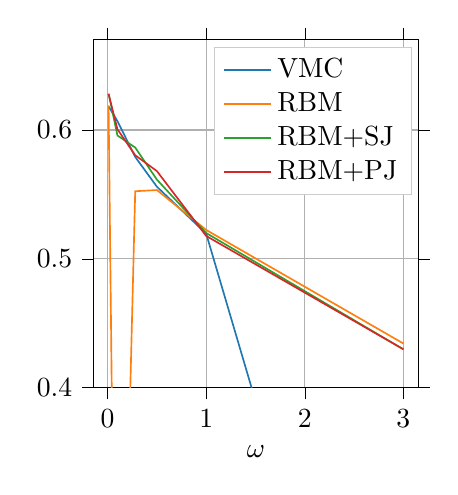
\begin{tikzpicture}

\definecolor{color0}{rgb}{0.12156862745098,0.466666666666667,0.705882352941177}
\definecolor{color1}{rgb}{1,0.498039215686275,0.0549019607843137}
\definecolor{color2}{rgb}{0.172549019607843,0.627450980392157,0.172549019607843}
\definecolor{color3}{rgb}{0.83921568627451,0.152941176470588,0.156862745098039}

\begin{axis}[
legend cell align={left},
legend style={draw=white!80.0!black},
tick align=outside,
tick pos=both,
x grid style={white!69.01960784313725!black},
xlabel={\(\displaystyle \omega\)},
xmajorgrids,
xmin=-0.1395, 
xmax=3.1495,
width=5.7cm,
height=6cm,
xtick style={color=black},
y grid style={white!69.01960784313725!black},
%ylabel={\(\displaystyle \langle\mathcal{V}_{int}\rangle/\langle\mathcal{H}\rangle\)},
ymajorgrids,
ymin=0.40, 
ymax=0.67,
ytick style={color=black}
]
\addplot [semithick, color0]
table {%
0.01 0.6182263233
0.1 0.606827096
0.28 0.579069037
0.5 0.555935404
1 0.519519289
3 0
};
\addlegendentry{VMC}
\addplot [semithick, color1]
table {%
0.01 0.619108895
0.1 0
0.28 0.5524393917
0.5 0.553357308
1 0.522390303
3 0.434265696
};
\addlegendentry{RBM}
\addplot [semithick, color2]
table {%
0.01 0.628145536
0.1 0.595709248
0.28 0.586340904
0.5 0.561447945
1 0.520004336
3 0.429762203
};
\addlegendentry{RBM+SJ}
\addplot [semithick, color3]
table {%
0.01 0.628019324
0.1 0.600510678
0.28 0.580389005
0.5 0.568074506
1 0.51773554
3 0.4297622035
};
\addlegendentry{RBM+PJ}
\end{axis}

\end{tikzpicture}}}
	\caption{In figure (a), the kinetic energy over total energy, $\langle\hat{T}\rangle/\langle\hat{H}\rangle$, of two-dimensional quantum dots containing 20 electrons are plotted as a function of the oscillator frequency $\omega$. Similar plots for the external potential energy and interaction energy are found in figure (b) and (c) respectively. The methods used were detailed in the introductory words of this chapter.}
	\label{fig:energysplit20}
\end{figure}
\fi 
\iffalse
\begin{table}
	\caption{This table shows how the total energy ($\langle\hat{H}\rangle$) is distributed between kinetic energy ($\langle\hat{T}\rangle$), external potential energy ($\langle\hat{V}_{\text{ext}}\rangle$) and interaction energy ($\langle\hat{V}_{\text{int}}\rangle$) of two-dimensional circular quantum dots at a wide range of frequencies $\omega$ and $N=12$ interacting electrons. The energy is given in units of $\hbar$, and the numbers in parenthesis are the statistical uncertainties in the last digit. For abbreviations see the text.}
	\label{tab:splitfrequencyQD12P}
	\begin{tabularx}{\textwidth}{R{0.5cm}rrcR{2.3cm}R{2.3cm}R{2.3cm}R{2.3cm}R{0.3cm}} \hline\hline
		&\makecell{\\ \phantom{$N$} \\ \phantom{=}} & $\omega$ && \multicolumn{1}{c}{$\langle \hat{H}\rangle$} & \multicolumn{1}{c}{$\langle \hat{T}\rangle$} & \multicolumn{1}{c}{$\langle \hat{V}_{\text{ext}} \rangle$} & \multicolumn{1}{c}{$\langle \hat{V}_{\text{int}} \rangle$} \\ \hline \\
		&RBM & 0.01 && 2.5106(8) & 0.0682(2) & 0.893(1) & 1.549(1) \\
		&& 2.0 && 115.214(5) & 20.760(6) & 43.69(1) & 50.764(7) \\
		&& 10.0 && 435.36(2) & 114.61(2) & 200.13(4) & 120.62(1) \\
 		\hline \\
		
		&RBM+SJ & 0.01 && 2.4950(5) & 0.07(2) & 0.845(4) & 1.58(2) \\
		&& 2.0 && 112.502(2) & 18.118(4) & 44.118(4) & 50.201(6) \\
		&& 10.0 && 415.384(7) & 108.57(2) & 181.90(3) & 124.92(1) \\
 		\hline \\
		
		&RBM+PJ & 0.01 && 2.5019(4) & 0.0699(2) & 0.893(1) & 1.539(1) \\
		&& 2.0 && 111.9426(5) & 17.817(3) & 46.532(4) & 47.593(3) \\
		&& 10.0 && 415.943(9) & 124.13(2) & 157.92(3) & 133.89(1) \\ 
		\hline \\
		
		&VMC & 0.01 && 2.4972(3) & 0.05506(2) & 0.858(1) & 1.584(1)\\
		&& 2.0 && 111.8377(3) & 19.678(2) & 41.349(3) & 50.811(2) \\
		&& 10.0 && \textcolor{red}{414.36(3)} & 116.0(2) & 168.9(3) & 129.4(1) \\
		\hline\hline
	\end{tabularx}
\end{table}
\fi

\begin{table}
	\caption{This table shows how the total energy ($\langle\hat{H}\rangle$) is distributed between kinetic energy ($\langle\hat{T}\rangle$), external potential energy ($\langle\hat{V}_{\text{ext}}\rangle$) and interaction energy ($\langle\hat{V}_{\text{int}}\rangle$) of two-dimensional circular quantum dots at a wide range of frequencies $\omega$ and $N=12$ interacting electrons. The energy is given in units of $\hbar$, and the numbers in parenthesis are the statistical uncertainties in the last digit. For abbreviations see the text.}
	\label{tab:splitfrequencyQD20P}
	\begin{tabularx}{\textwidth}{R{0.5cm}rrcR{2.3cm}R{2.3cm}R{2.3cm}R{2.3cm}R{0.3cm}} \hline\hline
		&\makecell{\\ \phantom{$N$} \\ \phantom{=}} & $\omega$ && \multicolumn{1}{c}{$\langle \hat{H}\rangle$} & \multicolumn{1}{c}{$\langle \hat{T}\rangle$} & \multicolumn{1}{c}{$\langle \hat{V}_{\text{ext}} \rangle$} & \multicolumn{1}{c}{$\langle \hat{V}_{\text{int}} \rangle$} \\ \hline \\
		&RBM & 0.01 && 6.217(2) & 0.1236(4) & 2.244(2) & 3.849(2) \\
		&& 2.0 && 269.086(8) & 43.262(8) & 95.17(2) & 130.65(1) \\
		&& 10.0 && 961.03(4) & 260.2(1) & 364.8(1) & 336.06(7) \\
		\hline \\
		
		&RBM+SJ & 0.01 && 6.239(2) & 0.1372(6) & 2.184(2) & 3.919(3) \\
		&& 2.0 && 265.66(9) & 39.31(8) & 95.78(1) & 130.57(2) \\
		&& 10.0 && 952.71(2) & 237.65(4) & 392.06(7) & 323.00(3) \\
		\hline \\
		
		&RBM+PJ & 0.01 && 6.210(1) & 0.1208(5) & 2.189(2) & 3.900(2) \\
		&& 2.0 && 262.598(1) & 34.758(6) & 108.546(9) & 119.293(7) \\
		&& 10.0 && 947.33(2) & 257.67(5) & 348.35(6) & 341.31(3) \\ 
		\hline \\
		
		&VMC & 0.01 && 6.2097(8) & 0.1005(4) & 2.270(3) & 3.839(3) \\
		&& 2.0 && 262.5339(9) & 38.402(3) & 95.681(7) & 128.451(5) \\
		&& 10.0 && 945.596(8) & 231.56(4) & 389.26(7) & 324.77(3) \\
		\hline\hline
	\end{tabularx}
\end{table}

\newpage
\subsection{Low frequency dots} \label{sec:lowfrequencies}
In section \ref{sec:onebodyresults}, we found the one-body density to be shape-invariant for large frequencies from around $\omega=0.28$. However, when we further decreased the frequency down to $\omega=0.1$ the density plots changed significantly and we got other extrema and so on. The aim of this section is to investigate the transitions between the various shapes with frequencies down to $\omega=0.01$. We start with looking at quantum dots with two electrons, where the one-body density for the frequencies $\omega=0.28$, 0.1 and 0.01 can be found in figure \eqref{fig:lowfreq2P} produced by RBM+PJ and VMC. Those methods were selected as they hitherto have shown the most promising results and we want to see if the RBM+PJ can reveal effects that the VMC is not able to capture.

\begin{figure}
	\centering
	\captionsetup[subfigure]{labelformat=empty}
	\subfloat{\raisebox{1.5cm}{\rotatebox[origin=t]{90}{RBM+PJ}}}\hspace{0.1cm}
	\subfloat{{\includegraphics[width=5.1cm]{/home/evenmn/VMC/plots/int1/onebody2/2D/2P/0.280000w/RBMPJ_ADAM_MC1048576.png}}}\hspace{-0.cm}
	\subfloat{{\includegraphics[width=5.1cm]{/home/evenmn/VMC/plots/int1/onebody2/2D/2P/0.100000w/RBMPJ_ADAM_MC1048576.png}}}\hspace{-0.cm}
	\subfloat{{\includegraphics[width=5.1cm]{/home/evenmn/VMC/plots/int1/onebody2/2D/2P/0.010000w/RBMPJ_ADAM_MC2pow28_smooth_blue_small.png}}}\\ [-0.cm]
	
	\subfloat{\raisebox{1.5cm}{\rotatebox[origin=t]{90}{VMC}}}\hspace{0.1cm}
	\subfloat[$\omega=0.28$]{{\includegraphics[width=5.1cm]{/home/evenmn/VMC/plots/int1/onebody2/2D/2P/0.280000w/VMC_ADAM_MC1048576.png}}}\hspace{-0.cm}
	\subfloat[$\omega=0.1$]{{\includegraphics[width=5.1cm]{/home/evenmn/VMC/plots/int1/onebody2/2D/2P/0.100000w/VMC_ADAM_MC1048576.png}}}\hspace{-0.cm}
	\subfloat[$\omega=0.01$]{{\includegraphics[width=5.1cm]{/home/evenmn/VMC/plots/int1/onebody2/2D/2P/0.010000w/VMC_ADAM_MC2pow28_smooth_blue_small.png}}}
	
	\caption{One-body density of two-dimensional circular quantum dots of frequencies $\omega=0.28$, 0.1 and 0.01 with $N=2$ electrons. The graph on the $yz$-plane represent the cross section through $x=0$. The surface plots are noise-reduced using a Savitzky-Golay filter, and for abbreviations see the text.}
	\label{fig:lowfreq2P}
\end{figure}

We see that the two methods obtain very similar density plots, where they agree that a ridge around center of the dot should be more distinct as the frequency drops. If we go back to figure \eqref{fig:energydistribution}, we saw that the kinetic energy was negligible for the lowest energies, and the effect is therefore an indication of the Wigner crystallization effect discussed in section \ref{sec:wigner}. Intuitively, the two electrons will repel each other and seldomly be located at the same place when their kinetic energy is low. RBM+PJ possibly provides a sharper plot for $\omega=0.01$, which is closer to the DMC results found in Ref.\cite{hogberget_quantum_2013} and thus perhaps more correct. Additionally, the ground-state energy obtained by RBM+PJ is lower than the energy obtained by VMC, with $E=0.074107(8)$ vs $E=0.074070(8)$ respectively. We repeat the exercise for quantum dots with six electrons, and obtain the plots in figure \eqref{fig:lowfreq6P}.

\begin{figure}
	\centering
	\captionsetup[subfigure]{labelformat=empty}
	\subfloat{\raisebox{1.5cm}{\rotatebox[origin=t]{90}{RBM+PJ}}}\hspace{0.1cm}
	\subfloat{{\includegraphics[width=5.1cm]{/home/evenmn/VMC/plots/int1/onebody2/2D/6P/0.280000w/RBMPJ_ADAM_MC1048576.png}}}\hspace{-0.cm}
	\subfloat{{\includegraphics[width=5.1cm]{/home/evenmn/VMC/plots/int1/onebody2/2D/6P/0.100000w/RBMPJ_ADAM_MC1048576.png}}}\hspace{-0.cm}
	\subfloat{{\includegraphics[width=5.1cm]{/home/evenmn/VMC/plots/int1/onebody2/2D/6P/0.010000w/RBMPJ_ADAM_MC1048576.png}}}\\ [-0.cm]
	
	\subfloat{\raisebox{1.5cm}{\rotatebox[origin=t]{90}{VMC}}}\hspace{0.1cm}
	\subfloat[$\omega=0.28$]{{\includegraphics[width=5.1cm]{/home/evenmn/VMC/plots/int1/onebody2/2D/6P/0.280000w/VMC_ADAM_MC1048576.png}}}\hspace{-0.cm}
	\subfloat[$\omega=0.1$]{{\includegraphics[width=5.1cm]{/home/evenmn/VMC/plots/int1/onebody2/2D/6P/0.100000w/VMC_ADAM_MC1048576.png}}}\hspace{-0.cm}
	\subfloat[$\omega=0.01$]{{\includegraphics[width=5.1cm]{/home/evenmn/VMC/plots/int1/onebody2/2D/6P/0.010000w/VMC_ADAM_MC2pow28_smooth}}}
	
	\caption{One-body density of two-dimensional circular quantum dots of frequencies $\omega=0.28$, 0.1 and 0.01 with $N=6$ electrons. The surface plots are noise-reduced using a Savitzky-Golay filter, and for abbreviations see the text.}
	\label{fig:lowfreq6P}
\end{figure}

We observe the same tendency as for the dots with two electrons, where we get an additional peak in the density plot as the frequency decreases. Again the RBM+PJ gives a more distinct peak than the VMC, which is closer to the DMC one-body density plot found from Ref.\cite{hogberget_quantum_2013}. This substantiates the presence of Wigner crystallization, where the configuration of lowest potential energy is found with an electron in the center of the dot and the remaining five electrons surrounding with the same distance to each other and to the center. In order to give a more qualitative comparison of the various methods, we also present the radial one-body density profile of the quantum dots of frequency $\omega=0.01$ with two and six electrons, see figure \eqref{fig:lowfreq}. 

\begin{figure}[H]
	\centering
	\captionsetup[subfigure]{labelformat=empty}
	\subfloat{{\includegraphics[width=\textwidth/2]{/home/evenmn/VMC/plots/int1/onebody/2D/2P/0.010000w/ADAM_MC1048576.png}}}
	\subfloat{{\includegraphics[width=\textwidth/2]{/home/evenmn/VMC/plots/int1/onebody/2D/6P/0.010000w/ADAM_MC1048576.png}}}
	
	\caption{One-body density of two-dimensional circular quantum dots of frequency $\omega=0.01$. The graph on the $yz$-plane represent the cross section through $x=0$. The surface plots are noise-reduced using a Savitzky-Golay filter, and for abbreviations see the text.}
	\label{fig:lowfreq}
\end{figure}

\iffalse
\subsection{$S\neq0$}
When the number of particles in the quantum dot is among the magic numbers presented in equation \eqref{eq:HOclosedshell}, the ground state is guaranteed to be found at $L=S=0$. However, if we want to look at dots of other sizes, this is often not true, and we will therefore look at some cases with $S\neq 0$. We will still stick to $L=0$ and closed shell systems.

Imagine a dot of four particles with $S=1$ (three have spin up and the last has spin down). The ground state is obviously found when a spin up and a spin down particle is in the lowest energy state, and the remaining particles are in the first excited energy state. Since the lowest states and the first excited states with spin up are filled up, this is a closed shell system.

Again, our results will be benchmarked to DMC, with references Ref.\cite{pederiva_diffusion_2000} and Ref.\cite{ghosal_incipient_2007}. The former reference also presents Hartree-Fock results which we also will use. 

The results are listed in table \eqref{tab:sneq0}, where we use a restricted Boltzmann machine with Padé-Jastrow factor (RBM+PJ) and standard variational Monte-Carlo (VMC). 

We find both the RBM+PJ and VMC to reproduce the reference energy in all the cases. 

\begin{table}
	\caption{The ground state energy of two-dimensional circular quantum dots of frequency $\omega$ for a given spin configuration ($L$,$S$). The results were obtained by a restricted Boltzmann machine with Padé-Jastrow factor (RBM+PJ) and standard variational Monte-Carlo (VMC). For reference, the Hartree-Fock limit results from Ref.\cite{pederiva_diffusion_2000} (HF) and diffusion Monte-Carlo results from Refs.\cite{pederiva_diffusion_2000},\cite{ghosal_incipient_2007} (DMC) are listed. All energies are given in units of $\hbar$, and the numbers in parenthesis are the statistical uncertainties in the last digit.}
	\label{tab:sneq0}
	\begin{tabularx}{\textwidth}{rrXrrXR{2.3cm}R{2.3cm}R{2.3cm}R{2.3cm}} \hline\hline
		\makecell{\\ $N$ \\ \phantom{=}} & \makecell{$\omega$} & \phantom{R} & $L$ & $S$ & \phantom{R} & \multicolumn{1}{c}{RBM+PJ} & \multicolumn{1}{c}{VMC} & \multicolumn{1}{c}{\makecell{HF\\ (Ref.\cite{pederiva_diffusion_2000})}} & \multicolumn{1}{c}{\makecell{DMC\\ (Ref.\cite{pederiva_diffusion_2000})$^a$\\ (Ref.\cite{ghosal_incipient_2007})$^b$}} \\ \hline \\
		4 & 0.28 && 0 & 1 && 3.7475(2) & 3.7711(5) & 3.9033 & 3.7135(3)$^a$\\ \\
		8 & 0.28 && 0 & 1 && 12.828(3) & 12.849(1) & 13.1887 & 12.6903(7)$^a$ \\
		& 0.25 && 0 & 1 && 11.807(1) & 11.852(1) & - & 11.6697(1)$^b$ \\ \\
		9 & 0.28 && 0 & 3/2 && 15.886(4) & 15.812(4) & 16.1544 & 15.4784(7)$^a$\\
		&3.0 && 0 & 3/2 && 97.164(4) & 96.936(7) & - & 97.0095(3)$^b$\\ \\
		11 & 0.28 && 0 & 1/2 && 22.285(2) & 22.252(1) & 22.8733 & 22.0750(4)$^a$ \\ \hline\hline
	\end{tabularx}
\end{table}
\fi

\newpage
\subsection{Large dots}
In order to test the code, we also decided to run for systems with $N>56$. This has no scientific significance, other than testing how far a VMC code can go. One thing is that the computations get extremely expensive as the number of particle increases, but also the standard error is assumed to increase due to.. This means that we cannot just crack up the wall clock time and wait when studying large systems, at some point the standard error gets insufficiently large and we need to further increase the number of Monte Carlo cycles. The learning rate also needs to be decreased as the system sizes increase, which requires more iterations.  We look at weakly interacting particles, so we will not get any relativistic effects even when adding many particles.

\begin{table}[H]
	\caption{Energy of large circular quantum dots, $\omega=1.0$. All energies are given in units of $\hbar$, and the numbers in parenthesis are the statistical uncertainties in the last digit. For abbreviations see the text.}
	\label{tab:largeQD}
	\begin{tabularx}{\textwidth}{R{1.6cm}R{2cm}R{2cm}R{3cm}R{3cm}} \hline\hline
		& \makecell{\\ \phantom{$N$}} & $N$ & RBM & VMC \\ \hline \\
		& 2D & 72 & 1355.37(2) & 1340.520(7) \\
		&& 90 & 2194.12(9) & 1990.89(2) \\
		& 3D & 70 & 1129.40(2) & 1108.950(4) \\
		\hline \hline
	\end{tabularx}
\end{table}

\begin{figure}[H]
	\centering
	\captionsetup[subfigure]{labelformat=empty}
	\subfloat{\includegraphics[scale=0.4]{/home/evenmn/VMC/plots/int1/onebody/2D/72P/1.000000w/ADAM_MC1048576.png}}
	\subfloat{\includegraphics[scale=0.4]{/home/evenmn/VMC/plots/int1/onebody/2D/90P/1.000000w/ADAM_MC2pow28.png}}\\
	\subfloat[VMC, 72P]{\includegraphics[scale=0.4]{/home/evenmn/VMC/plots/int1/onebody2/2D/72P/1.000000w/VMC_ADAM_MC2pow28_blue.png}}
	\subfloat[RBM, 72P]{\includegraphics[scale=0.4]{/home/evenmn/VMC/plots/int1/onebody2/2D/72P/1.000000w/VMC_ADAM_MC2pow28_smooth_blue_masked.png}}
	\caption{One-body density of large circular quantum dots with frequency $\omega=1.0$. The graph on the $yz$-plane represent the cross section through $x=0$. The methods were detailed in the introductory words to this chapter, and the surface plots were noise-reduced using a Savitzky-Golay filter, and for abbreviations see the text.}
	\label{fig:largedotsOB}
\end{figure}

\iffalse
\begin{figure}[H]
	\centering
	\subfloat[RBM]{\includegraphics[scale=0.4]{/home/evenmn/VMC/plots/int1/twobody/2D/72P/1.000000w/RBM_ADAM_MC2pow28.png}}
	\subfloat[VMC]{\includegraphics[scale=0.4]{/home/evenmn/VMC/plots/int1/twobody/2D/72P/1.000000w/RBM_ADAM_MC2pow28.png}}
	\caption{One-body density of large two-dimensional circular quantum dots with frequency $\omega=1.0$ containing 72 particles.}
	\label{fig:largedotsTB}
\end{figure}
\fi

\iffalse
\section{Double quantum dots}
Double quantum dots are systems that are very interesting when it comes to testing the Boltzmann machines. Even though we know the wave functions for the non-interacting case, they are expansions that are computational expensive to work with.

\subsection{Ground state energy}
For the interacting case, we will use Alocias Mariadason's VMC calculations with and without a Hartree-Fock basis as a reference. In addition, Jørgen Høgberget provides a DMC energy for the case with two particles and $\omega=1.0$. All the results are given in table \eqref{tab:doubleQD}.
\begin{table}
	\caption{Double quantum dots. F is the number of functions used in the expansion.}
	\label{tab:doubleQD}
	\begin{tabularx}{\textwidth}{rrXR{2.3cm}R{2.3cm}R{2.3cm}R{2.3cm}R{2.3cm}} \hline\hline
		\makecell{\\ $N$ \\ \phantom{=}} & $\omega$ & \phantom{R} & \multicolumn{1}{c}{VMC (F=1)} & \multicolumn{1}{c}{RBM+PJ} & \multicolumn{1}{c}{\makecell{VMC (F$>$1)\\ (Ref.\cite{mariadason_quantum_2018})}} & \multicolumn{1}{c}{\makecell{VMC+HF\\ (Ref.\cite{mariadason_quantum_2018})}} & \multicolumn{1}{c}{\makecell{DMC\\ (Ref.\cite{hogberget_quantum_2013})}} \\ \hline \\
		2 & 0.1 && 0.41982(4) & 0.41939(3)\\
		& 0.28 && 0.9365(1) & 0.92618(4) \\
		& 0.5 && 1.4847(2) & 1.44004(4) \\
		& 1.0 && 2.6331(5) & 2.38342(3) & 2.42238(4) & 2.36618(4) & 2.3496(1) \\ \hline \\
		
		4 & 0.1 \\
		& 0.28 \\
		& 0.5 \\
		& 1.0 && - & - & 7.95247(4) & 7.90232(4) & - \\ \hline \\
		
		6 & 0.1 \\
		& 0.28 \\
		& 0.5 \\
		& 1.0 && - & - & 16.61419(4) & 16.55609(4) \\ \hline \\
		
		8 & 0.1 \\
		& 0.28 \\
		& 0.5 \\
		& 1.0 && - & - & \\ \hline \hline
	\end{tabularx}
\end{table}
What we observe, is that the Boltzmann machine with a Padé-Jastrow factor outperforms a Hermite expansion of 10 functions, which is surprising. The reason might be that the Boltzmann machine consists of a sum over all hidden nodes, which makes it behave similar to an expansion. However, the Boltzmann machine was then again beat by the Hermite expansion with a Hartree-Fock basis. 
\fi

\newpage
\section{Atoms}
The next systems we will address are the real atomic systems, which have been investigated by physicists since the childhood of quantum mechanics. This section is added just to show the flexibility of the implemented code, which can easily be expanded to new systems. We use the simple Hydrogen-like orbitals in our calculations, detailed in section \ref{sec:atomic}. In table \ref{tab:atomswinteraction} we present the ground state energy of the four smallest closed-shell atoms Helium, Beryllium, Neon and Magnesium, including an overview of how the energy is distributed and the ratio between kinetic and potential energy. We also compare the obtained results to experimental values. What we see, is that the total energy is similar, but slightly higher than our reference, which is as expected as we use a simple basis.

If we once again recall the virial theorem first introduced in section \ref{sec:virial}, it reads
\begin{empheq}[box={\mybluebox[5pt]}]{equation}
2\langle\hat{T}\rangle = -(\langle\hat{V}_{\text{ext}}\rangle + \langle\hat{V}_{\text{int}}\rangle)
\end{empheq}
for atoms and molecules. Taking the ratio between the kinetic and potential energy should therefore give $\langle\hat{T}\rangle/\langle\hat{V}\rangle=-0.5$, which is almost what we obtain. We therefore have a reason to believe that the energies are calculated correctly. 

\begin{table}
	\caption{Energy of neutral atoms of atomic number $Z$ produced by VMC. We present the total energy ($\langle\hat{H}\rangle$), the external potential energy ($\langle\hat{V}_{\text{ext}}\rangle$), the interaction energy ($\langle\hat{V}_{\text{int}}\rangle$), the kinetic-potential energy ratio ($\langle\hat{T}\rangle/\langle\hat{V}\rangle$) and experimental values (Expr.). The latter were taken from Ref.\cite{degroote_faddeev_2013}, table 4.4. The energy is given in atomic units, and the numbers in parenthesis is the statistical error. For abbreviations see the text.}
	\label{tab:atomswinteraction}
	\begin{tabularx}{\textwidth}{lrrR{2cm}R{1.9cm}|R{1.8cm}R{1.8cm}R{1.8cm}R{1.7cm}} \hline\hline
		Atom & $Z$ & \makecell{\\ \phantom{=} \\ \phantom{=}} & 
		\multicolumn{1}{c}{\makecell{Expr.\\ (Ref.\cite{degroote_faddeev_2013})}} & \multicolumn{1}{c}{$\langle\hat{H}\rangle$} & \multicolumn{1}{c}{$\langle\hat{T}\rangle$} & \multicolumn{1}{c}{$\langle\hat{V}_{\text{ext}}\rangle$} & \multicolumn{1}{c}{$\langle\hat{V}_{\text{int}}\rangle$} & \multicolumn{1}{c}{$\langle\hat{T}\rangle/\langle\hat{V}\rangle $} \\ \hline \\
		
		He & 2 && -2.9037 & -2.8719(3) & 2.813(3) & -6.696(4) & 1.010(7) & -0.495 \\
		Be & 4 && -14.6674 & -14.4992(5) & 15.465(6) & -34.987(7) & 5.023(1) & -0.516 \\
		Ne & 10 && -128.9383 & -128.09(1) & 133.4(2) & -318.4(2) & 56.94(5) & -0.510 \\ 
		Mg & 12 && -200.054 & -196.81(4) & 251.9(2) & -557.0(2) & 108.23(6) & -0.379 \\ \hline\hline
	\end{tabularx}
\end{table}
\begin{figure}
	\centering
	\captionsetup[subfigure]{labelformat=empty}
	\subfloat[Helium]{\includegraphics[width=\textwidth/2]{/home/evenmn/VMC/plots/int1/atoms/He/ADAM_MC2pow28.png}}
	\subfloat[Beryllium]{\includegraphics[width=\textwidth/2]{/home/evenmn/VMC/plots/int1/atoms/Be/ADAM_MC2pow28.png}}\\
	\subfloat[Neon]{\includegraphics[width=\textwidth/2]{/home/evenmn/VMC/plots/int1/atoms/Ne/ADAM_MC2pow28.png}}
	\subfloat[Magnesium]{\includegraphics[width=\textwidth/2]{/home/evenmn/VMC/plots/int1/atoms/Mg/ADAM_MC2pow28.png}}
	\caption{Radial one-body density plots obtained for the Helium atom (upper left), the Beryllium atom (upper right), the Neon atom (lower left) and the Magnesium atom (lower right). VMC was used, which is detailed in the text. The number of Monte Carlo cycles used was $M=2^{28}=268,435,456$.}
	\label{fig:atomsonebody}
\end{figure}
Further, we look at the one-body densities, which are presented in figure \eqref{fig:atomsonebody} for our four atoms. To reveal details, they are multiplied with $r^2$ as for example J.Høgberget has done before us \cite{hogberget_quantum_2013}. We observe that the densities also are similar to his DMC results, which again substantiates that our framework and electron density computations work as they should. 
